\documentclass{article}
\usepackage{graphicx} % Required for inserting images
\usepackage{amsmath}
\usepackage[english, russian] {babel}
\usepackage[utf8]{inputenc}
\usepackage[T2A]{fontenc}
\usepackage{minted}
\usepackage{float}
\usepackage{amssymb}

\title{Формальные языки программирвонаия}
\author{silvia.lesnaia }
\date{February 2025}

\begin{document}

\maketitle


\textbf{13.02.25}
\section{Введение в компиляторы}
\section{Теория формальных языков и трансляций}
    \subsection{Введение в компиляторы}

    Языки высокого уровня

    \hspace{50mm} $\leftarrow$ Трансляторы(компиляторы)

    Ассемблеры

    Машинные языки
    \subsection{ВВЕДЕНИЕ}
    
\begin{figure}[H]
    \centering
    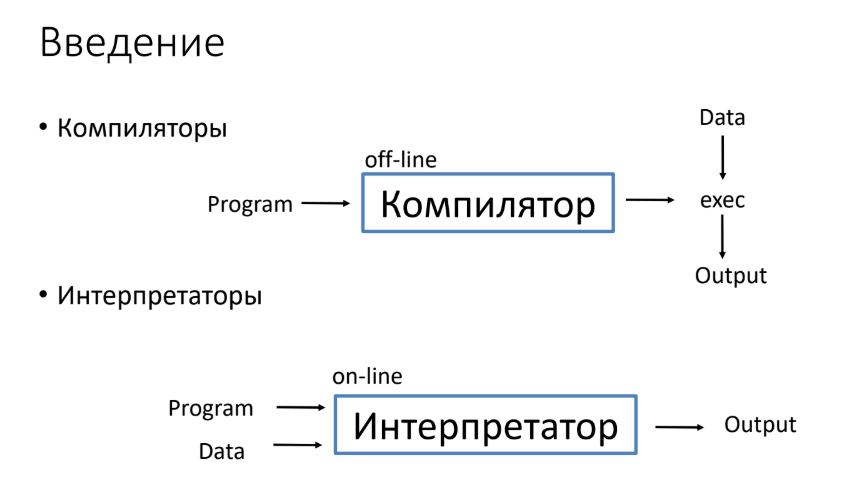
\includegraphics[width=1\linewidth]{Снимок экрана 2025-02-13 083445.png}
\end{figure}

    \subsubsection{Процесс компиляции}
    
    \begin{figure}[H]
        \centering
        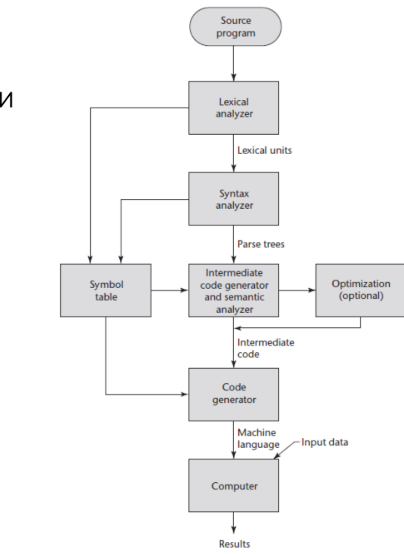
\includegraphics[width=1\linewidth]{Снимок экрана 2025-02-13 083723.png}
    \end{figure}

    \begin{figure}[H]
        \centering
        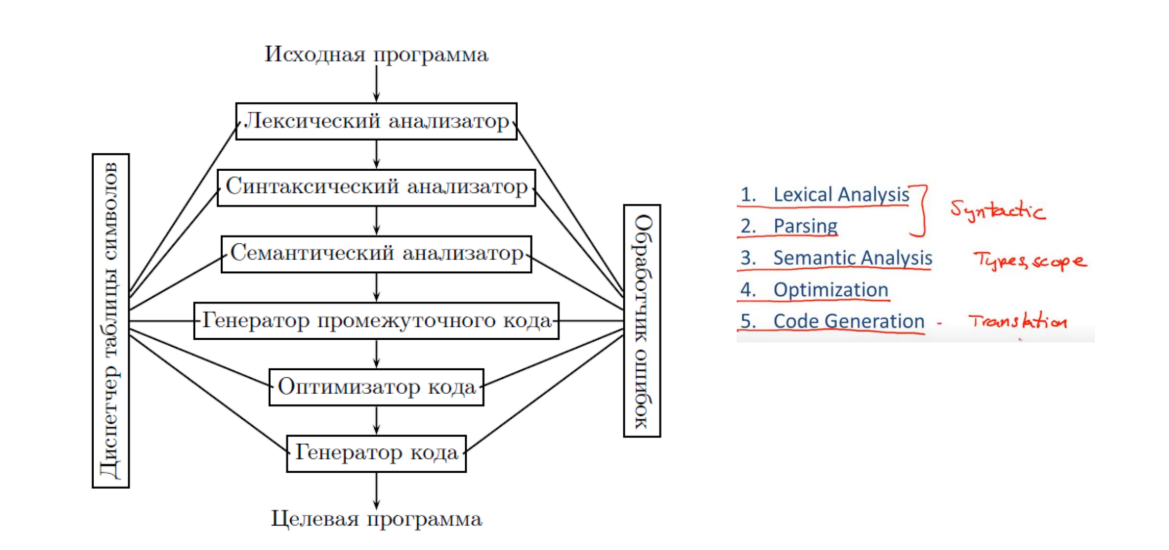
\includegraphics[width=1\linewidth]{Снимок экрана 2025-02-13 084306.png}
    \end{figure}

• 1. Лексический анализ – деление текста на слова, выделение
«токенов»

• This is a sentence

• Thi sis ase nte nce

• if x==y then z=1; else z=2;

\begin{figure}[H]
    \centering
    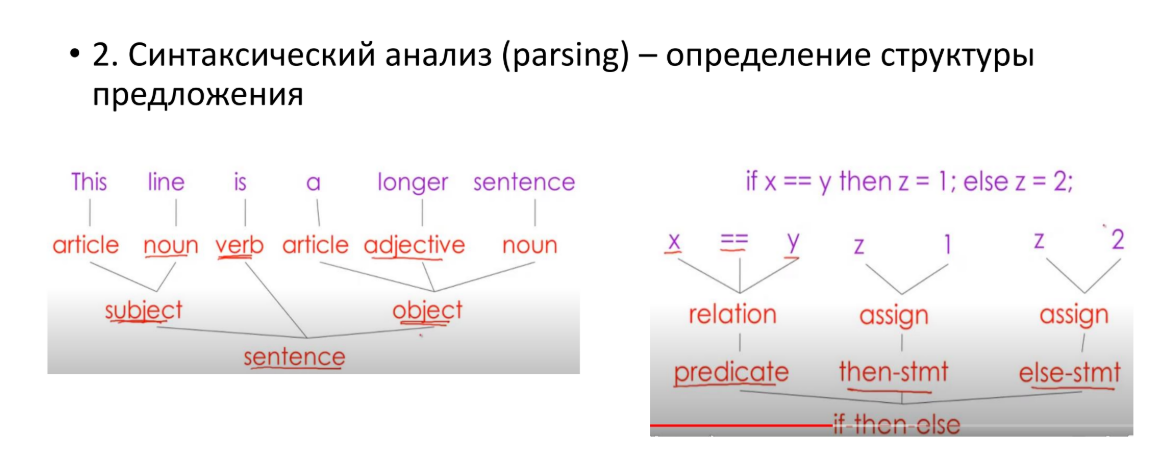
\includegraphics[width=1\linewidth]{Снимок экрана 2025-02-13 084508.png}
\end{figure}

• 3. Семантический анализ (устранение неоднозначностей)
• Пример:

• Петя сказал Мите оставить его задание дома

• Более сложный пример:

• Петя сказал Пете оставить его задание дома

• Языки программирования определяют строгие правила избегания
двусмысленности

{

int Jack = 3;

{

int Jack =4;

cout << Jack;

}

}

Компиляторы выполняют множество семантических проверок
относительно переменных

• Пример:

• Петя оставил её задание дома

• Из-за «несоответствия типов» между «её» и «Петя» мы узнаём,
что это разные люди.

• 4. Оптимизация кода

• На естественном языке оптимизация не имеет строгих правил и
сводится к редактированию.

• Для программы: Автоматическая модификация, чтобы:
• Работать быстрее

• Использовать меньше памяти

• (энергосбережение, сети, БД)

• X=Y*0

• X=0

• 5. Генерация кода

• Обычно результатом является ассемблерный код
или

• Трансляция на другой язык программирования

• Общая структура почти всех компиляторов соответствует нашему
описанию

• Пропорции в объеме вычислений в процессе трансляции
изменились:

\begin{figure}[H]
    \centering
    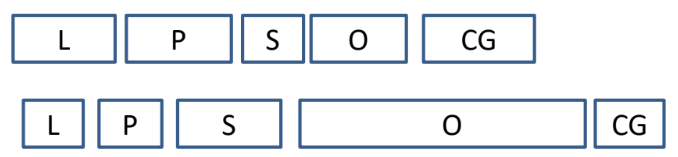
\includegraphics[width=0.5\linewidth]{Снимок экрана 2025-02-13 085253.png}
\end{figure}

\begin{figure}[H]
    \centering
    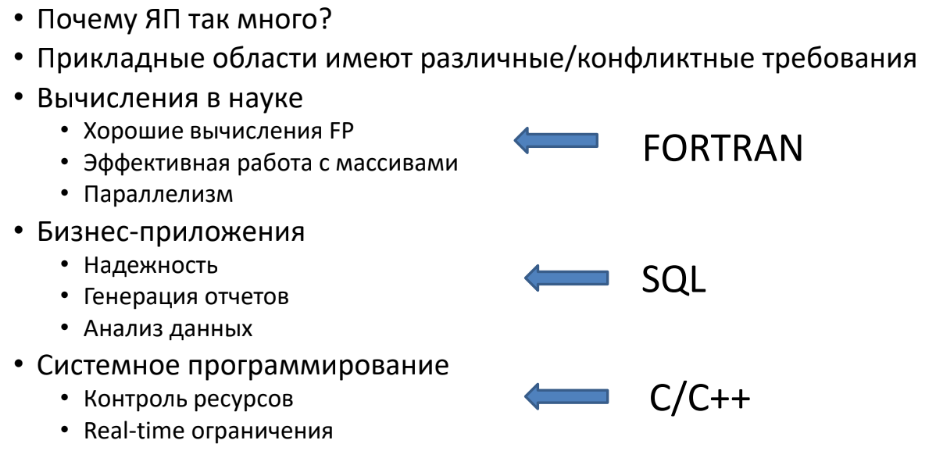
\includegraphics[width=1\linewidth]{Снимок экрана 2025-02-13 085330.png}
\end{figure}

\begin{figure}[H]
    \centering
    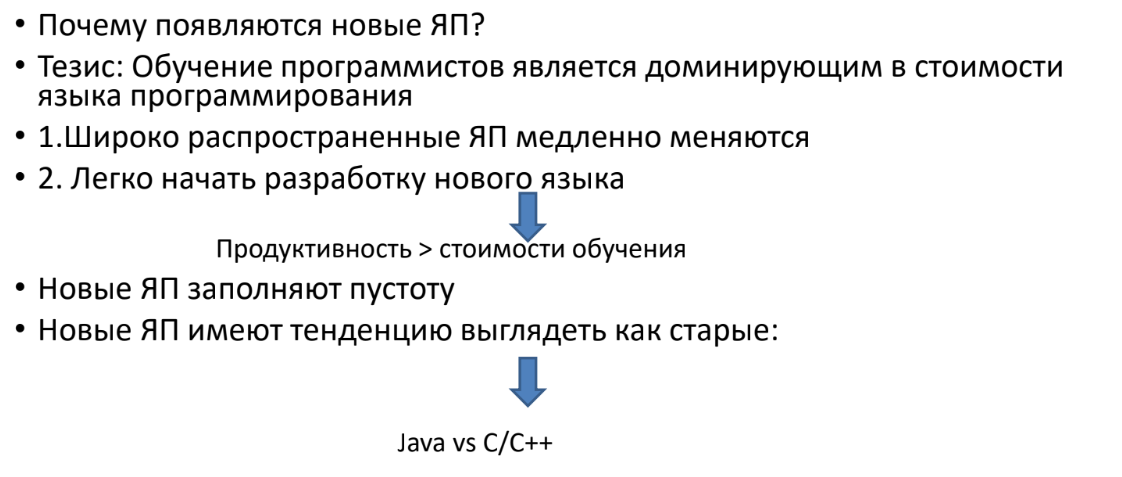
\includegraphics[width=1\linewidth]{Снимок экрана 2025-02-13 085352.png}
\end{figure}

\subsection{Лексический анализ}

• Просмотр потока символов программы (слева направо) и выделение
лексических единиц – токенов

position := initial + rate * 60

position – идентификатор

:= - операция

initial - идентификатор

+ - операция

rate - идентификатор

* - операция

60 - число (целое)

\begin{figure}[H]
    \centering
    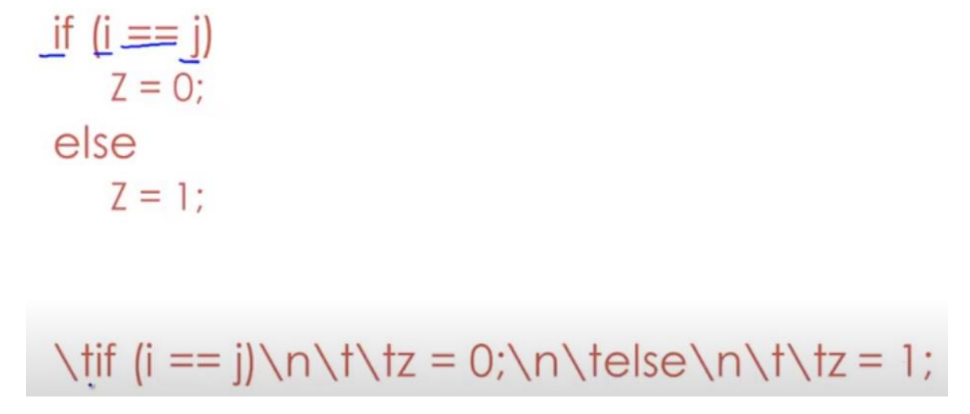
\includegraphics[width=1\linewidth]{Снимок экрана 2025-02-13 090554.png}
\end{figure}

• Классам токенов соответствуют множества строк
• Примеры:

• Идентификатор ::= строка букв и цифр, начинающаяся с буквы

• Целое число ::= непустая строка цифр

• Ключевое слово ::= < if | then | else | while | for | ...>

• Пробел ::= непустая последовательность кодов символов для
пробела новой строки, табуляции

\begin{figure}[H]
    \centering
    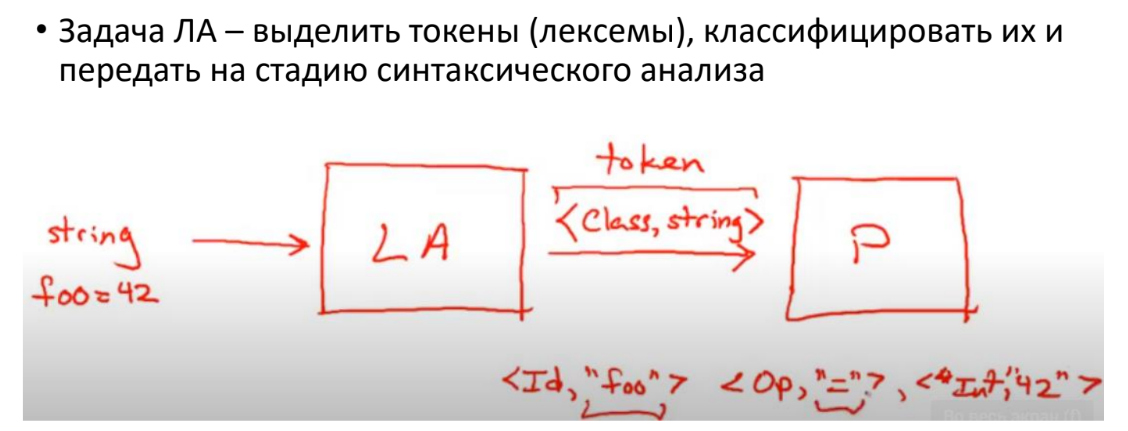
\includegraphics[width=1\linewidth]{Снимок экрана 2025-02-13 090702.png}
\end{figure}

if (i==j)

z=0;

else

z=1

\begin{figure}[H]
    \centering
    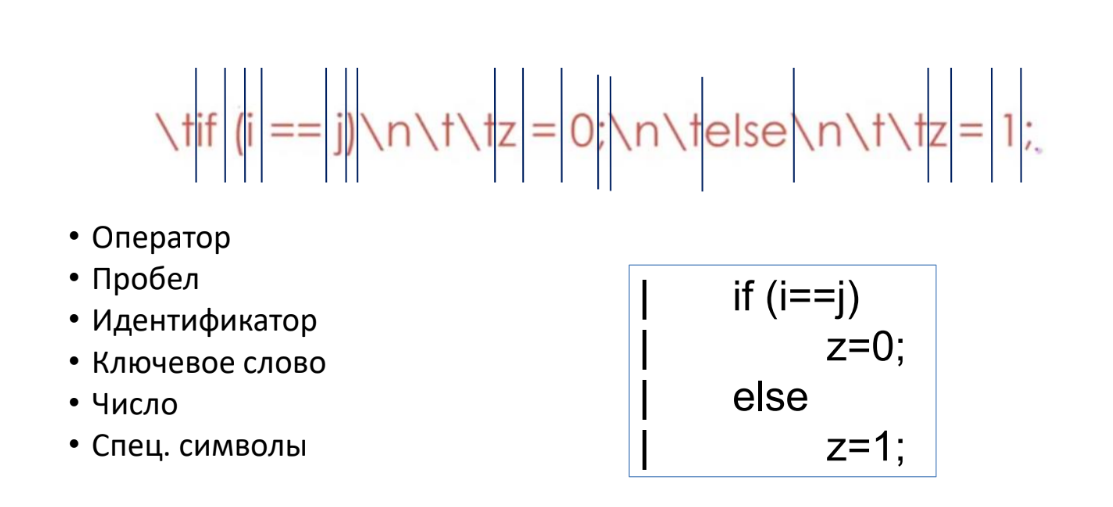
\includegraphics[width=1\linewidth]{Снимок экрана 2025-02-13 090834.png}
\end{figure}

• Примеры

• FORTRAN – пробелы не учитываются

• VAR1 – то же самое, что VA R1

• DO 5 i=1,25

• DO 5 i=1.25

• Необходимо заглядывать при просмотре строки вперёд

\begin{figure}[H]
    \centering
    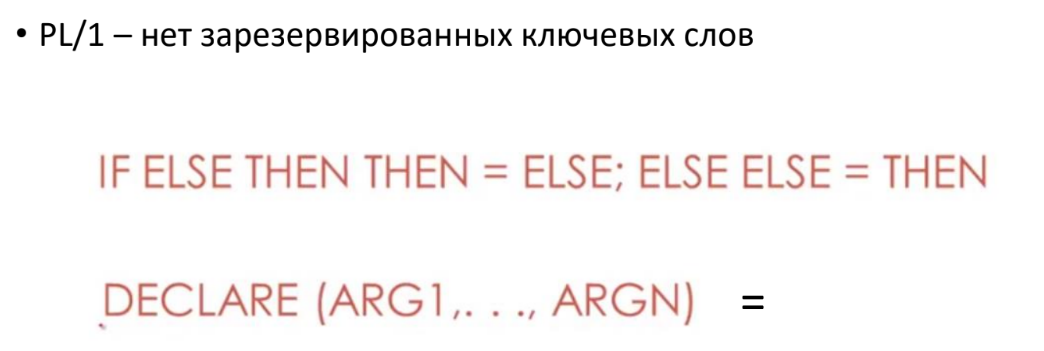
\includegraphics[width=1\linewidth]{Снимок экрана 2025-02-13 091234.png}
\end{figure}


• С++

• Синтакс :

• Foo<Bar>

• cin>>Bar

• Foo<Bar<Bazz>>

\subsection{Синтаксический анализ}

\begin{figure}[H]
    \centering
    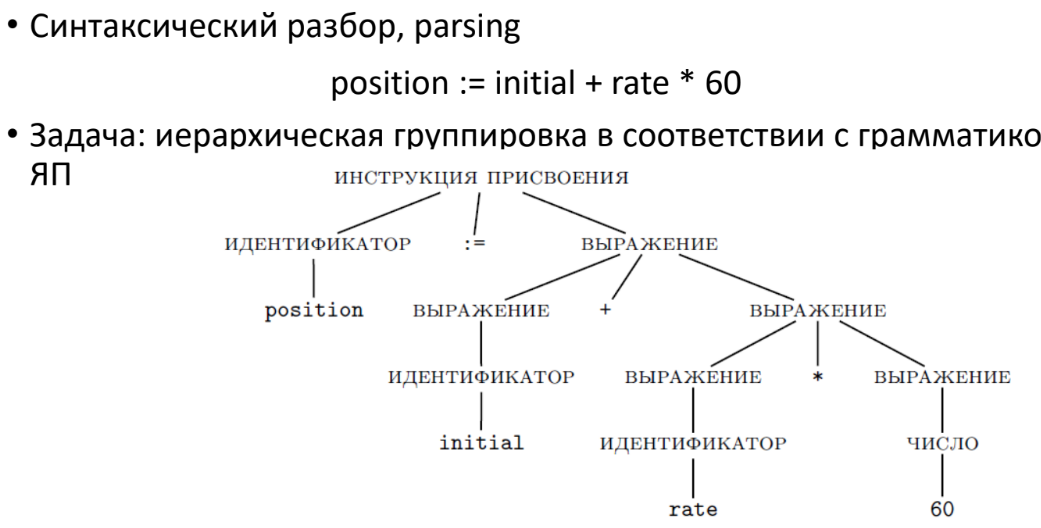
\includegraphics[width=1\linewidth]{Снимок экрана 2025-02-13 091654.png}
\end{figure}

\begin{figure}[H]
    \centering
    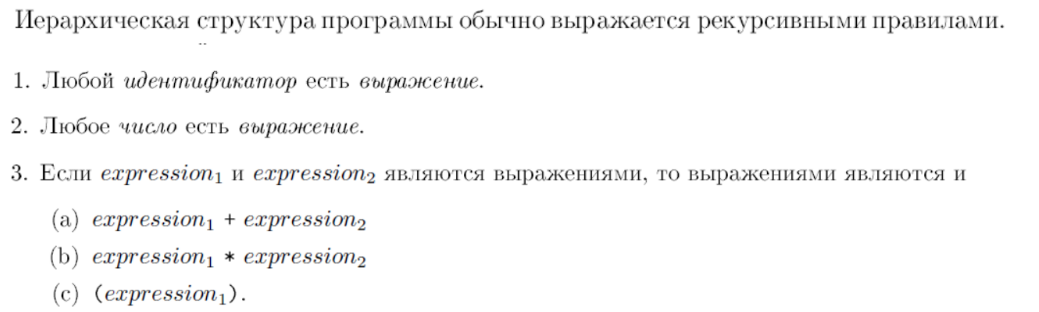
\includegraphics[width=1\linewidth]{Снимок экрана 2025-02-13 091754.png}
    \end{figure}
    
    \subsection{Семантический анализ}
    
\begin{figure}[H]
    \centering
    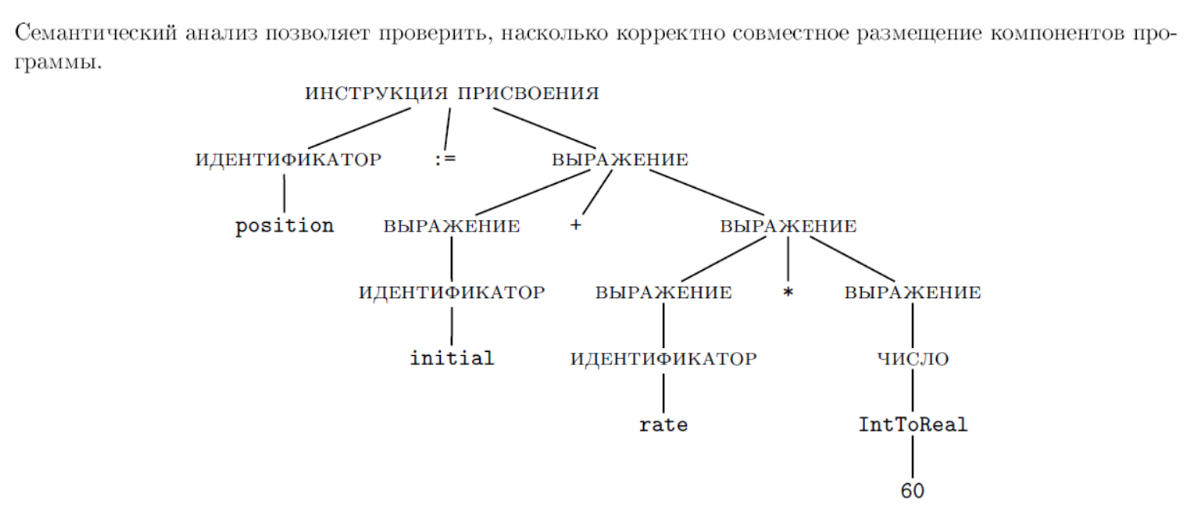
\includegraphics[width=1\linewidth]{Снимок экрана 2025-02-13 091809.png}
\end{figure}

\subsection{Генерация промежуточного кода}

\begin{figure}[H]
    \centering
    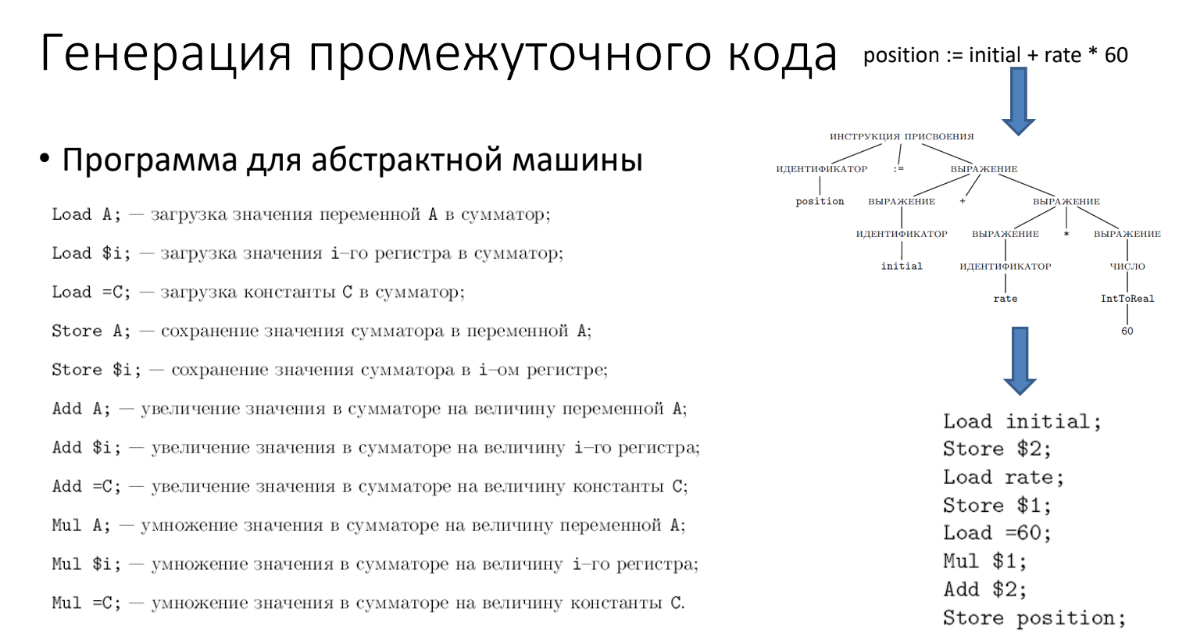
\includegraphics[width=1\linewidth]{Снимок экрана 2025-02-13 092347.png}
\end{figure}

\subsection{Зависимость от архитектуры компьютера}
\begin{figure}[H]
    \centering
    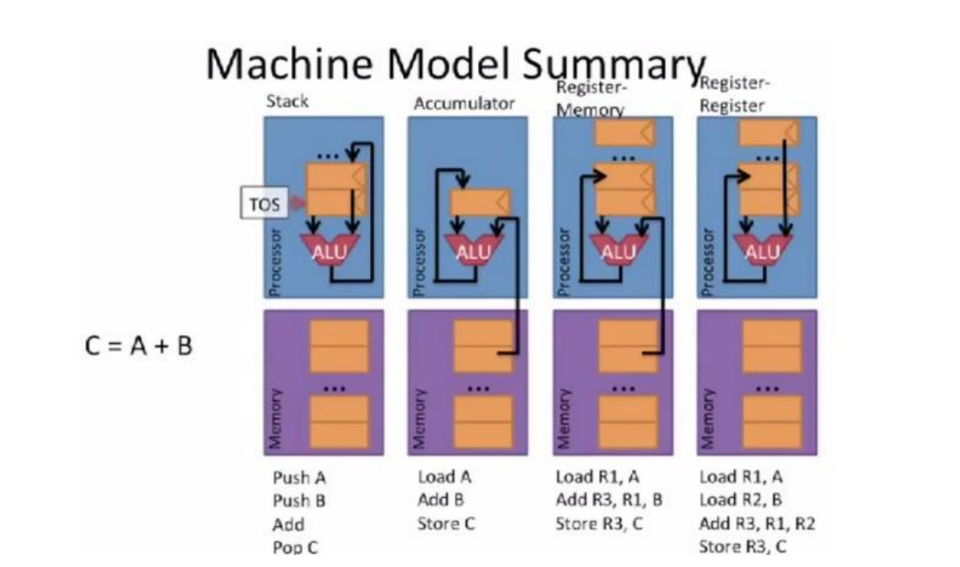
\includegraphics[width=1\linewidth]{Снимок экрана 2025-02-13 092401.png}
\end{figure}

\subsection{Оптимизация кода}

\begin{figure}[H]
    \centering
    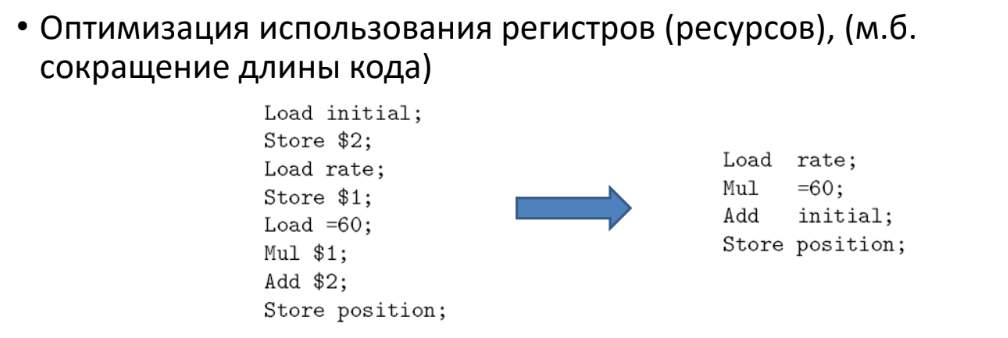
\includegraphics[width=1\linewidth]{Снимок экрана 2025-02-13 093155.png}
\end{figure}

\subsection{Генерация целевого кода}

\begin{figure}[H]
    \centering
    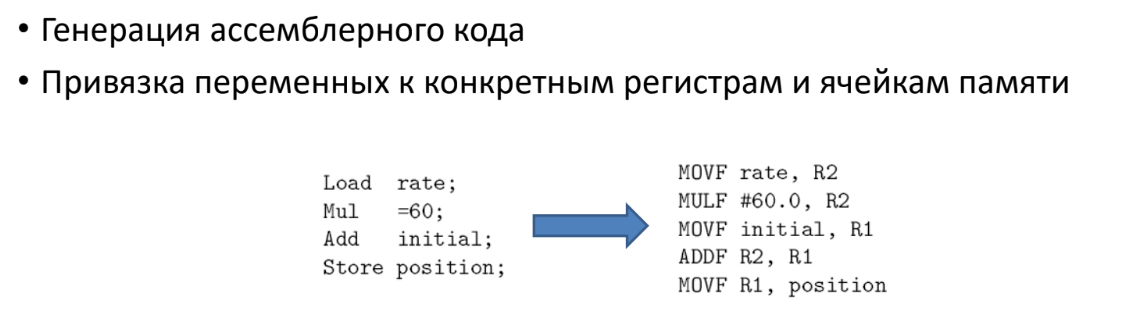
\includegraphics[width=1\linewidth]{Снимок экрана 2025-02-13 093218.png}
\end{figure}

\section{Формальные языки}

\subsection{Основные понятия и определения формальных языков}

• Опр. Алфавит — это конечное множество символов.

• Опр. Цепочкой символов (или словом) в алфавите $\Sigma$ называется любая конечная
последовательность символов этого алфавита.

• Опр. Цепочка, которая не содержит ни одного символа, называется пустой
цепочкой. Обозначение: $\epsilon$ (в алфавит $\Sigma$ не входит, она лишь помогает обозначить
пустую последовательность символов).

• Опр. Если a и b — цепочки, то цепочка ab (результат приписывания цепочки b в
конец цепочки a), называется конкатенацией (или сцеплением) цепочек a и b.
Конкатенацию можно считать двуместной операцией над цепочками: a×b = ab.

Например, если w = ab и z = cd, то w×z = abcd.

Для любой цепочки a : a$\epsilon$ = $\epsilon$a = a.

• Для любых цепочек a, b, g справедливо свойство ассоциативности операции конкатенации (ab)g = a(bg) = abg.

\subsection{Операции над цепочками символов}

\begin{figure}[H]
    \centering
    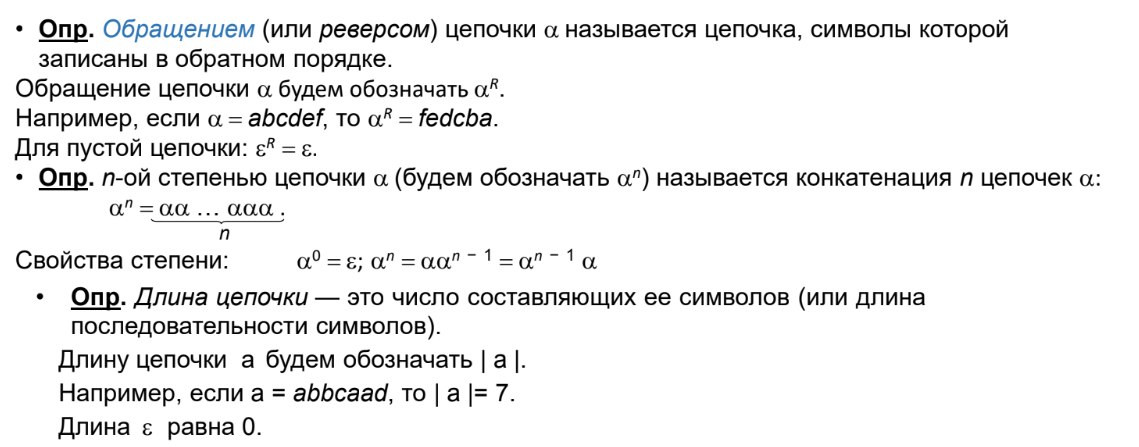
\includegraphics[width=1\linewidth]{Снимок экрана 2025-02-13 093643.png}
\end{figure}

\begin{figure}[H]
    \centering
    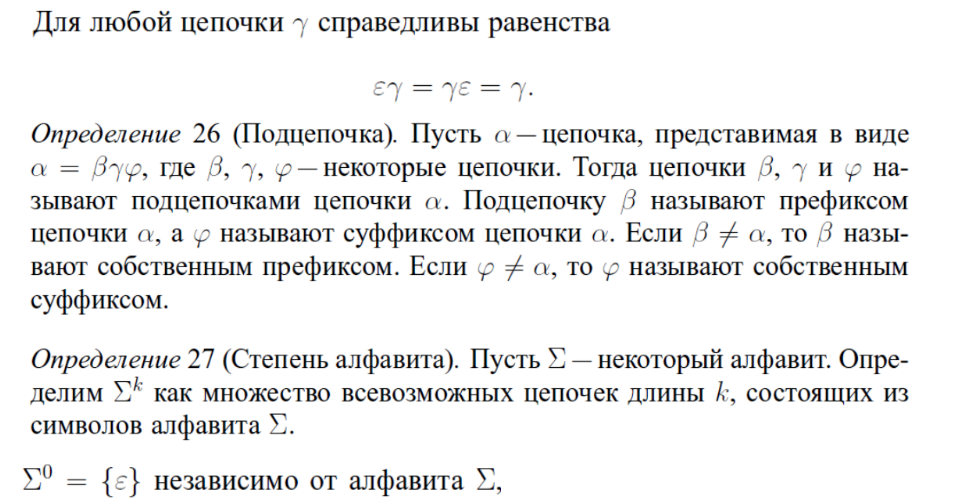
\includegraphics[width=1\linewidth]{Снимок экрана 2025-02-13 093853.png}
\end{figure}

\subsection{Формальный язык}
\begin{figure}[H]
    \centering
    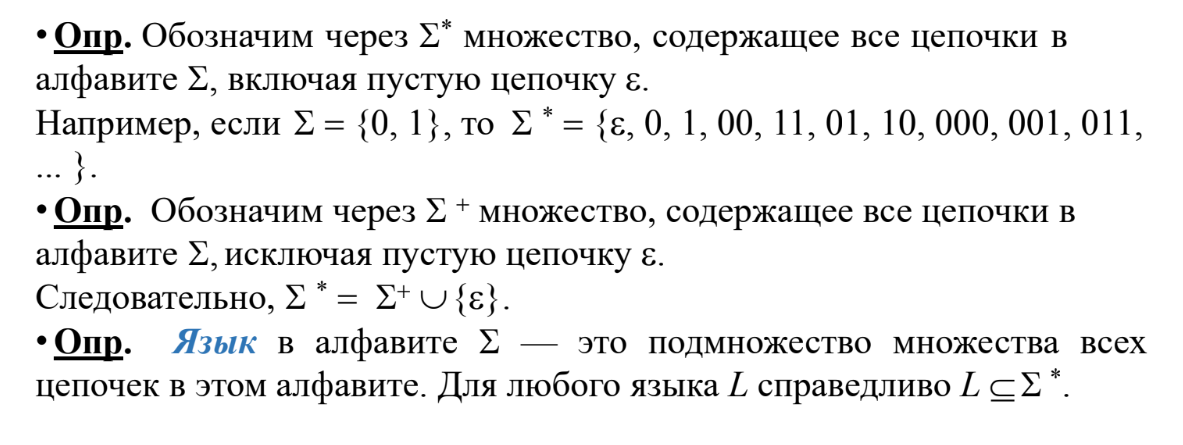
\includegraphics[width=1\linewidth]{Снимок экрана 2025-02-13 094552.png}
\end{figure}

\textbf{20.02.25}

\section{Формальный язык}


\begin{figure}[H]
    \centering
    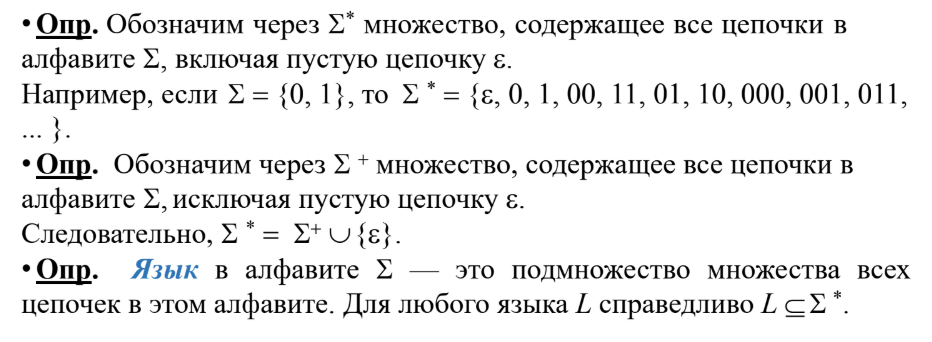
\includegraphics[width=1\linewidth]{image.png}
\end{figure}

Примеры

1. L = {$\varepsilon$, 01, 0011, 000111, 00001111, . . .} - язык над алфавитом
{0, 1}, в котором цепочки состоят из последовательностей k
единиц вслед за k нулями (k $\geq$ 0).
2. L = {$\varepsilon$}. Язык в любом алфавите, состоящий только из пустого
слова
3. L = $\varnothing$ Пустой язык в любом алфавите.
4. L = {$\varepsilon$, 01, 10, 0011, 1100, 1001, 0110, 0101, . . .} язык над
алфавитом {0, 1}, в котором равное число нулей и единиц.

\section{Операции над языками}
\begin{figure}[H]
    \centering
    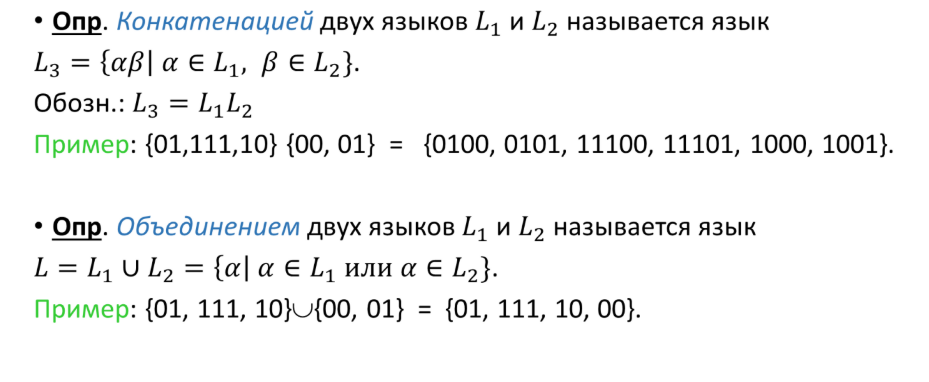
\includegraphics[width=1\linewidth]{Снимок экрана 2025-02-20 084202.png}
\end{figure}

\begin{figure}[H]
    \centering
    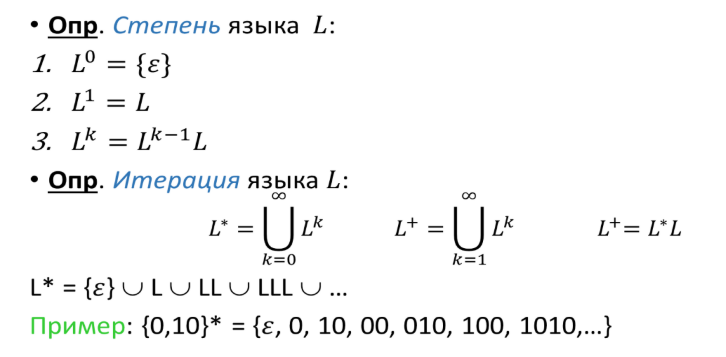
\includegraphics[width=1\linewidth]{Снимок экрана 2025-02-20 084233.png}
\end{figure}


\section{Способы описания языков}

• Конечный язык можно описать простым перечислением его
цепочек.

• Как представлять бесконечные языки?

• спецификация (описание)

• механизм распознавания

• механизм порождения (генерации).

• Не каждый формальный язык можно задать с помощью конечного
описания.


• Спецификация – Описание языка, как множества слов,
удовлетворяющих некоторому условию. (Для регулярных языков – это
регулярное выражение.

• Механизм распознавания (распознаватель), по сути, является
процедурой специального вида, которая по заданной цепочке
определяет, принадлежит ли она языку.

• Если принадлежит, то процедура останавливается с ответом «да», т. е.
допускает цепочку; иначе — останавливается с ответом «нет» или
зацикливается.

• Язык, определяемый распознавателем — это множество всех
цепочек, которые он допускает.

• Основной способ реализации механизма порождения —
использование порождающих грамматик

\section{Грамматики}

\begin{figure}[H]
    \centering
    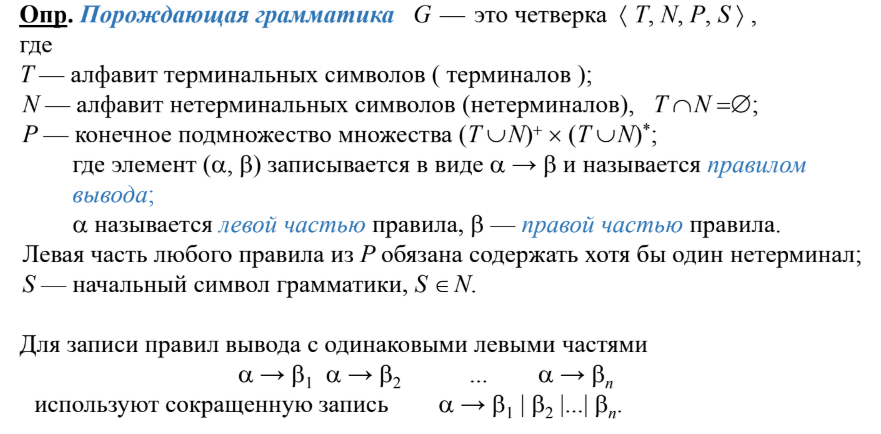
\includegraphics[width=1\linewidth]{Снимок экрана 2025-02-20 084954.png}
\end{figure}

Пример
$G_example$ = $\langle$ {0, 1}, {A, S}, P, S $\rangle$

P: S → 0A1

0A → 0A1

A → e

\section{Выводимость цепочки}

\begin{figure}[H]
    \centering
    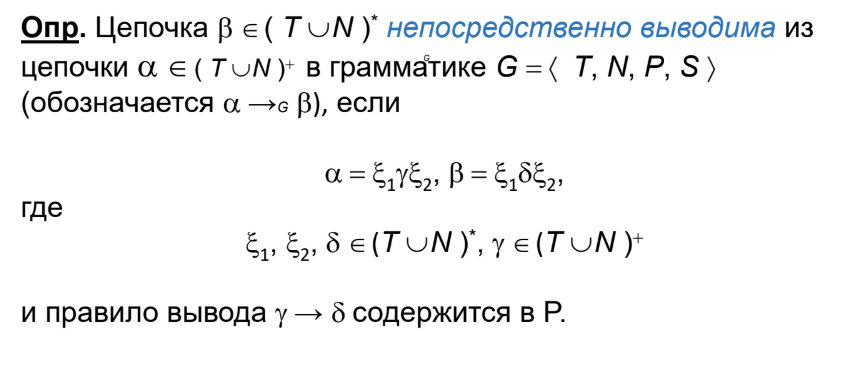
\includegraphics[width=1\linewidth]{Снимок экрана 2025-02-20 090552.png}
    
\end{figure}

\begin{figure}[H]
    \centering
    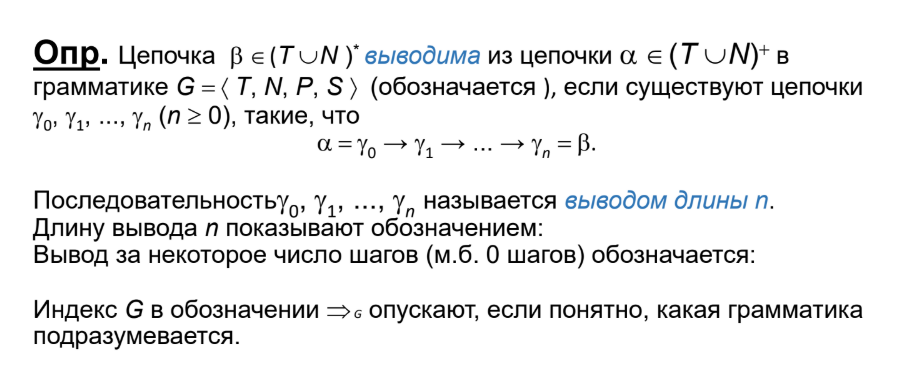
\includegraphics[width=1\linewidth]{Снимок экрана 2025-02-20 090612.png}
\end{figure}

\section{Язык грамматики}

\begin{figure} [H]
    \centering
    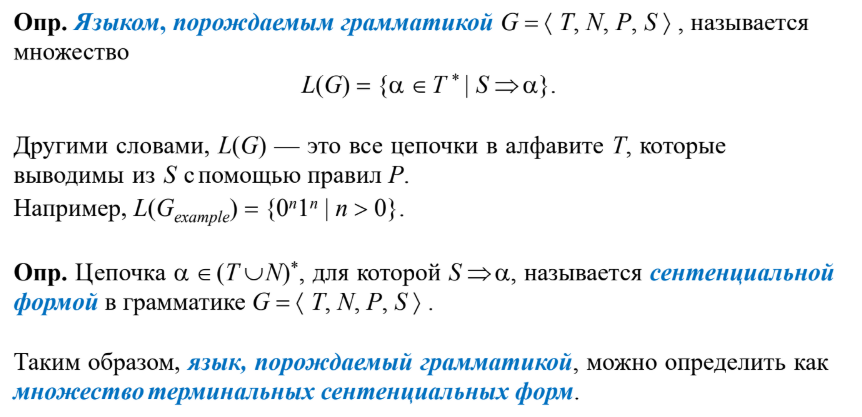
\includegraphics[width=1\linewidth]{Снимок экрана 2025-02-20 091501.png}
\end{figure}

\begin{figure}[H]
    \centering
    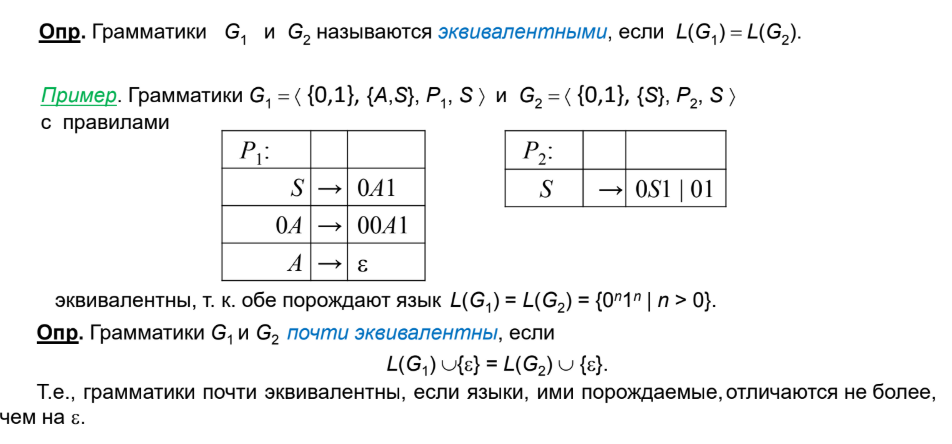
\includegraphics[width=1\linewidth]{Снимок экрана 2025-02-20 091507.png}
\end{figure}


\section{Распознаватель}
• Механизм, который является процедурой специального вида, которая по
заданной цепочке определяет, принадлежит ли она языку.

• Если принадлежит, то процедура останавливается с ответом «да», т. е.
допускает цепочку; иначе — останавливается с ответом «нет» или
зацикливается.

• Язык, определяемый распознавателем — это множество всех цепочек,
которые он допускает.

\begin{figure}[H]
    \centering
    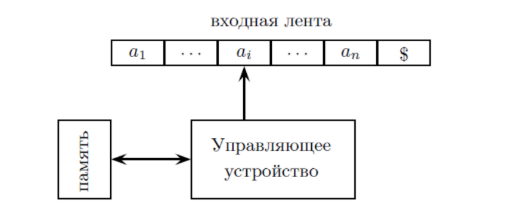
\includegraphics[width=0.5\linewidth]{Снимок экрана 2025-02-20 091653.png}
\end{figure}

\section{Классификация грамматик и языков по Хомскому}


• Тип грамматики определяется типом ограничений на вид
правил вывода.

• Всего определено четыре типа грамматик:
тип 0, тип 1, тип 2, тип 3.

• Каждому типу грамматик соответствует свой класс
языков.

• Если язык порождается грамматикой типа i (для i = 0, 1, 2,
3), то он является языком типа i.

\subsection{Классификация грамматик и языков по
Хомскому: Тип 0}

\textbf{Тип 0}

Любая порождающая грамматика является грамматикой
типа 0.

На вид правил грамматик этого типа не накладывается
никаких дополнительных ограничений.

Класс языков типа 0 совпадает с классом рекурсивно
перечислимых языков.

\subsection{Классификация грамматик и языков по
Хомскому: Тип 1}

Опр. Грамматика G = $\langle$ T, N, P, S $\rangle$ называется неукорачивающей, если
правая часть каждого правила из P не короче левой части (т. е. для
любого правила a → b $\epsilon$ P выполняется неравенство | a | $\leq$ | b | ).

В виде исключения в неукорачивающей грамматике допускается
наличие правила S → e, при условии, что S (начальный символ) не
встречается в правых частях правил.

Грамматикой типа 1 называют неукорачивающую грамматику.
\begin{figure}[H]
    \centering
    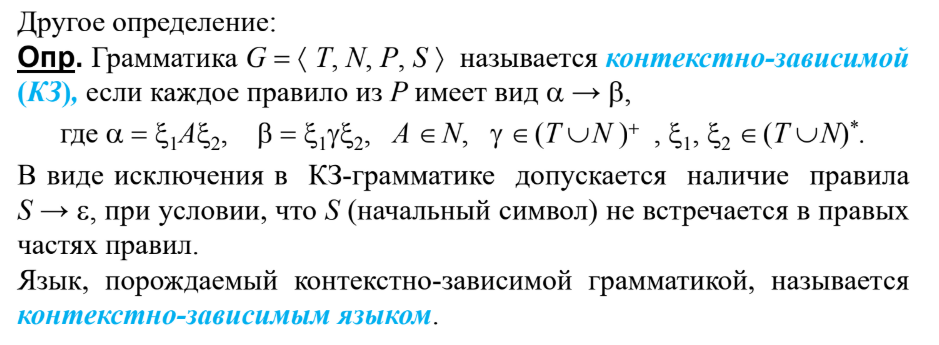
\includegraphics[width=1\linewidth]{Снимок экрана 2025-02-20 092937.png}
\end{figure}

\subsubsection{}{Эквивалентность неукорачивающих и
КЗ-грамматик}

Утверждение 1. Пусть L — формальный язык. Следующие утверждения
эквивалентны.
1) существует контекстно-зависимая грамматика $G_1$, такая что $L = L(G_1)$

2) существует неукорачивающая грамматика G2, такая что $L = L(G_2).$

Док-во. Очевидно, что (1) $\implies$ (2): любая контекстно-зависимая грамматика удовлетворяет ограничениям неукорачивающей грамматики (см. определения).

Т.к. каждое неукорачивающее правило можно заменить эквивалентной
серией контекстно-зависимых правил, следовательно (2) $\implies$ (1).

\subsection{Классификация грамматик и языков по
Хомскому: Тип 2}

Опр. Грамматика G = $\langle$ T, N, P, S $\rangle$ называется контекстно-свободной (КС),
если каждое правило из Р имеет вид A → b, где A $\varepsilon$N, b $\varepsilon$( T $\cup$ N )*.

Заметим, что в КС-грамматиках допускаются правила с пустыми правыми
частями. Язык, порождаемый контекстно-свободной грамматикой,
называется контекстно-свободным языком.
Грамматикой типа 2 будем называть контекстно-свободную грамматику.

КС-грамматика может являться неукорачивающей, т.е. удовлетворять
ограничениям неукорачивающей грамматики.

Утверждение 2. Для любой КС-грамматики G существует
неукорачивающая КС- грамматика G', такая что L(G) = L(G').

\subsection{Классификация грамматик и языков по
Хомскому: Тип 3}


\begin{figure}[H]
    \centering
    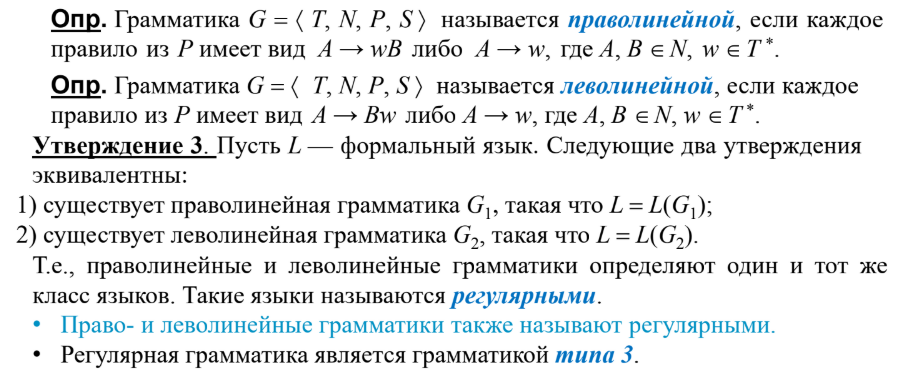
\includegraphics[width=1\linewidth]{Снимок экрана 2025-02-20 094134.png}
\end{figure}

\subsection{Автоматные грамматики}

Опр. Автоматной грамматикой называется праволинейная (леволинейная)
грамматика, такая, что каждое правило с непустой правой частью имеет вид:
A → a либо A → aB (для леволинейной, соответственно, A → a либо A → Ba),
где A, B $\epsilon$N, a $\epsilon$T.

Автоматная грамматика является более простой формой регулярной грамматики.

Существует алгоритм, позволяющий по регулярной (право- или леволинейной) грамматике построить соответствующую автоматную грамматику.

Таким образом, любой регулярный язык может быть порожден автоматной
грамматикой.

Существует алгоритм, позволяющий устранить из регулярной (автоматной)
грамматики все e-правила (кроме S → e в случае, если пустая цепочка принадлежит языку; при этом S не будет встречаться в правых частях правил).

Утверждение 4. Для любой регулярной (автоматной) грамматики G существует неукорачивающая регулярная (автоматная) грамматика G'
, такая что $L(G) = L(G')$.

\subsection{Иерархия грамматик Хомского}

Утверждение 5. Справедливы следующие утверждения:
1) любая регулярная грамматика является КС-грамматикой;
2) любая неукорачивающая КС-грамматика является КЗ-грамматикой;
3) любая неукорачивающая грамматика является грамматикой типа 0.

Утверждение 5 следует непосредственно из определений.

Рассматривая только неукорачивающие регулярные и неукорачивающие КС-
грамматики, получаем следующую иерархию классов грамматик:

Регулярные неукорачивающие $\subset$ КС неукорачивающие $\subset$ КЗ $\subset$ Тип 0

\section{Иерархия языков}

Утверждение 6. Справедливы следующие утверждения:
1) Каждый регулярный язык является КС-языком, но существуют КС-языки,
которые не являются регулярными, например:

$L = \{ a^n b^n | n  > 0 \}  $

2) Каждый КС-язык является КЗ-языком, но существуют КЗ-языки,
которыене являются КС-языками, например:

$ L = \{a^n b^n c^n | n > 0\}; $

3) Каждый КЗ-язык является языком типа 0 (т. е. рекурсивно перечислимым
языком), но существуют языки типа 0, которые не являются КЗ-языками.
Из утверждения 6 следует иерархия классов языков:

Тип 3 (Регулярные) $\subset$ Тип 2 (КС)  $\subset$ Тип 1 (КЗ)  $\subset$ Тип 0

\begin{figure}[H]
    \centering
    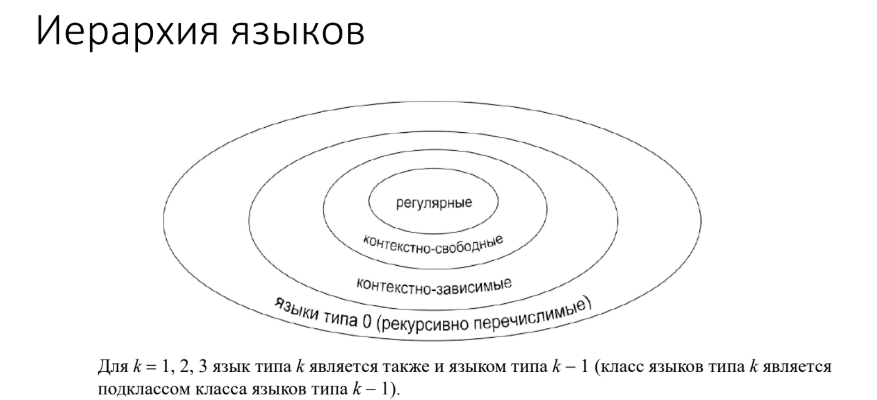
\includegraphics[width=1\linewidth]{Снимок экрана 2025-02-27 084055.png}
\end{figure}


• Утверждение 7. Проблема «Можно ли язык, описанный
грамматикой типа k (k = 0, 1, 2), описать грамматикой типа k + 1?»
является алгоритмически неразрешимой.

• Т.е., нет алгоритма, позволяющего по заданному описанию языка L
(например, по грамматике), определить максимальное k, такое что L
является языком типа k

• НО! В примерах и задачах при ответе на вопрос «Какого типа заданный
язык L?» будем указывать, если не оговорено иное, максимально
возможное k для заданного языка L.

\textbf{27.02.25}

\section{Разбор цепочек}

Опр. Цепочка в алфавите T принадлежит языку, порождаемому грамматикой
$ \langle  T, N, P, S \rangle $ , только в том случае, если существует ее вывод из начального
символа S этой грамматики.

• Процесс построения такого вывода (а, следовательно, и определения
принадлежности цепочки языку) называется разбором.
• Построение вывода можно осуществлять и в обратном порядке: в исходной
цепочке ищем вхождение в неё правой части некоторого правила и заменяем
егона левую часть (делаем свёртку).

• В итоге исходная цепочка «сворачивается» к некоторой сентенциальной
форме. Затем идет следующая свертка и т. д., пока не придем к S .
• Такой процесс разбора называют также анализом.

\begin{figure}[H]
    \centering
    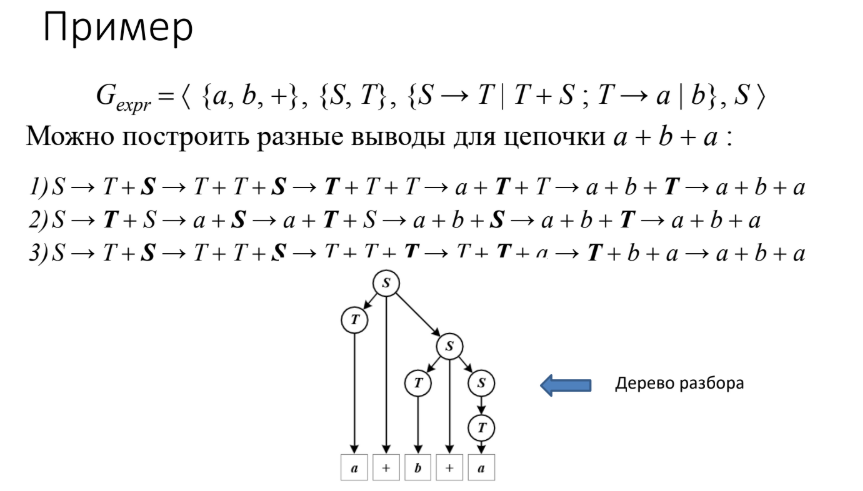
\includegraphics[width=1\linewidth]{Снимок экрана 2025-02-27 084444.png}
\end{figure}

\section{Регулярные множества, их распознавание и порождение}

\subsection{Регулярные множества и регулярные выражения}

• Опр. Пусть $\Sigma$ - конечный алфавит. Регулярное множество в
алфавите $\Sigma$ определяется следующим образом:
1) $\varnothing$ - регулярное множество в алфавите $\Sigma$.

2) $\{\epsilon\} $- регулярное множество в алфавите $\Sigma$.

3) $\{\alpha\}$ - регулярное множество в алфавите $\Sigma$ для каждого $\alpha \in  \Sigma$.

4) Если Q и P - регулярные множества в алфавите $\Sigma,$ то множества
Q $\cup$ P , QP и P* регулярные.

5) Ничто другое не является регулярным множеством в алфавите $\Sigma$.

\subsection{Регулярные выражения}


Опр. Пусть $\Sigma$ — конечный алфавит. Определим рекурсивно регулярное
выражение в алфавите $\Sigma$ и регулярные множества, которые они обозначают.
Базис индукции:

1) $\varnothing$ есть регулярное выражение, обозначающее регулярное множество $\varnothing$

2) $\epsilon$ есть регулярное выражение, обозначающее регулярное множество $\{\epsilon\} $

3) $\alpha \in \Sigma$  есть регулярное выражение, обозначающее регулярное множество $\{\alpha\}$
Индукция:

Если $\alpha$ и $\beta$ — регулярные выражения, обозначающие регулярные множества Q$\cup $P соответственно, то:

1) ($\alpha + \beta $) — регулярное выражение, обозначающее Q$\cup$P;

2) ($\alpha \beta $) — регулярное выражение, обозначающее QP;

3) ($\beta$)*

* — регулярное выражение, обозначающее P*;

Никаких других регулярных выражений, кроме тех, что построены в
соответствии с описанным определением, нет.


\begin{figure}[H]
    \centering
    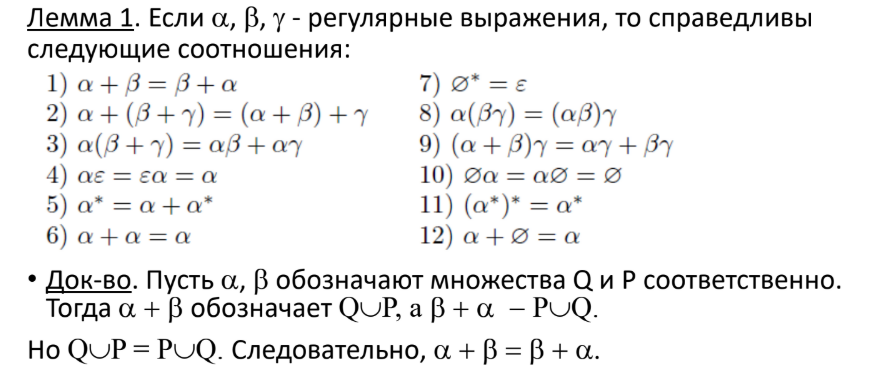
\includegraphics[width=1\linewidth]{Снимок экрана 2025-02-27 085900.png}
\end{figure}



\subsection{Алгебраические законы для регулярных
выражений}
• Объединение и конкатенация ведут себя как сложение и
умножение.

• + является коммутативным и ассоциативным;

• Конкатенация является ассоциативной операцией.

• Конкатенация распределяется по +.

• Исключение: Конкатенация не коммутативна.

\subsection{Единицы и нейтральные элементы в RE}

• $\varnothing$ является нейтральным элементом для +.
R + $\varnothing$ = R.

• e является «единицей» для конкатенации.
$\epsilon R = R\epsilon = R.$

• $\varnothing $ является «нулем» для конкатенации.
$\varnothing R = R \varnothing = \varnothing.$

\textbf{Пример преобразования RE}

!ЭТА ЗАДАЧА БУДЕТ В кр

\begin{figure}[H]
    \centering
    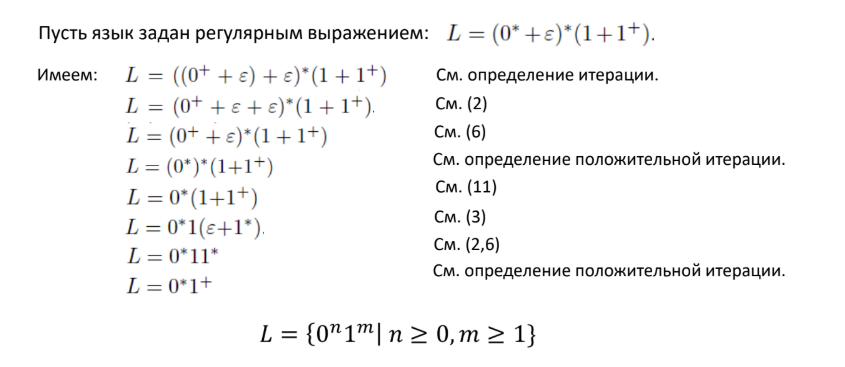
\includegraphics[width=1\linewidth]{Снимок экрана 2025-02-27 090738.png}
\end{figure}


\textbf{Примеры RE}


• $\Sigma=\{0,1\}$

• $ L(01) = \{01\}.$

• $L(01+0) = \{01, 0\}.$

• $L(0(1+0)) = \{01, 00\}.$

• $ L(0*) = \{\epsilon, 0, 00, 000,... \}.$

• $ L((0+10)*(\epsilon+1))$ = все строки из 0 и 1 без двух последовательных 1.
 

\begin{figure}[H]
    \centering
    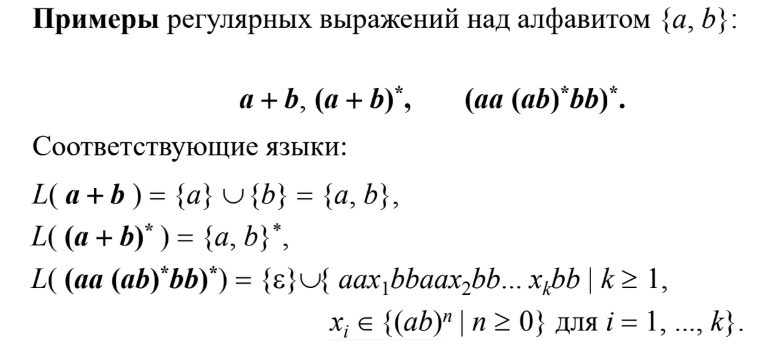
\includegraphics[width=1\linewidth]{Снимок экрана 2025-02-27 091410.png}
\end{figure}

\subsection{Уравнения с регулярными коэффициентами}

• Рассм. уравнение X=aX+b, где a и b – РВ.
X=a*b – решение уравнения:

a*b=aa*b+b

a*b=(aa*+e)b

a*b=a*b

Если множество, определяемое рег. выражением a, содержит e, то
ур-е имеет бесконечно много решений: X=a*(b+c) для любого РВ c.
В этом случае берут «наименьшее решение» – наименьшую
неподвижную точку.


\textbf{06.03.25}

\section{Регулярные множества и праволинейные грамматики}

\begin{figure}[H]
    \centering
    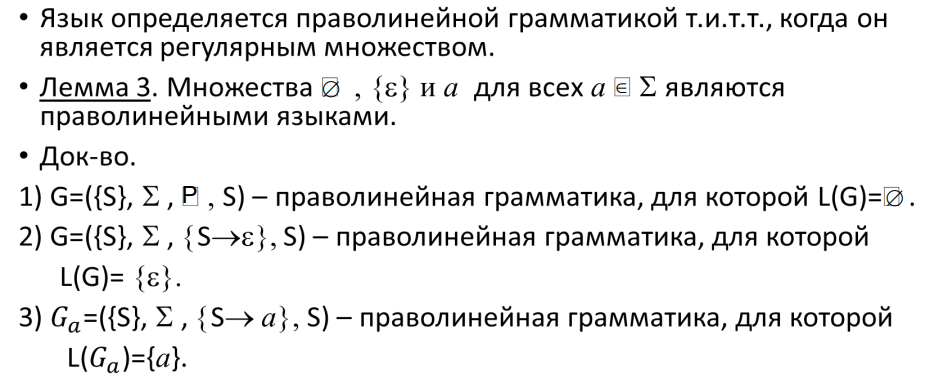
\includegraphics[width=1\linewidth]{Снимок экрана 2025-03-06 082915.png}
\end{figure}


\begin{figure}[H]
    \centering
    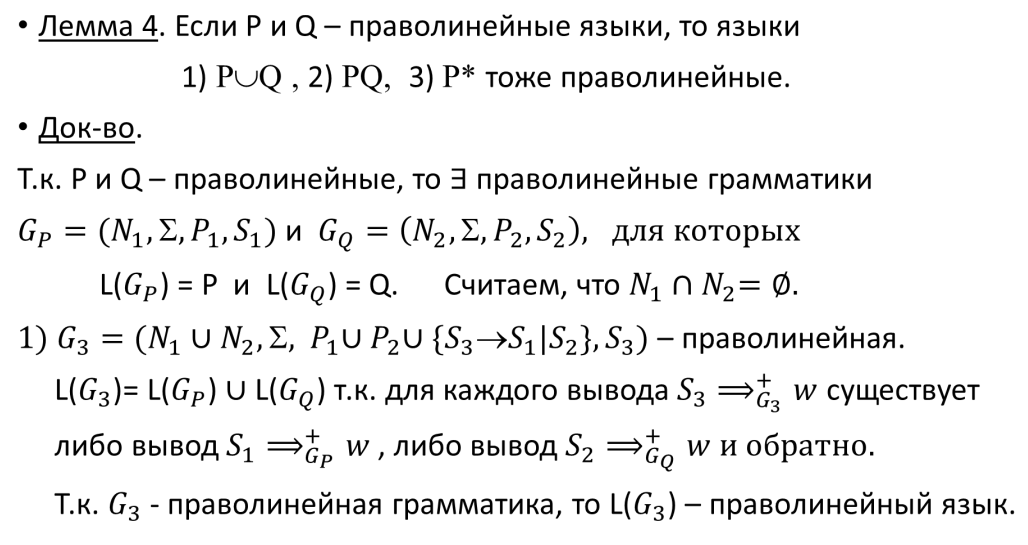
\includegraphics[width=1\linewidth]{Снимок экрана 2025-03-06 083016.png}
\end{figure}


\begin{figure}[H]
    \centering
    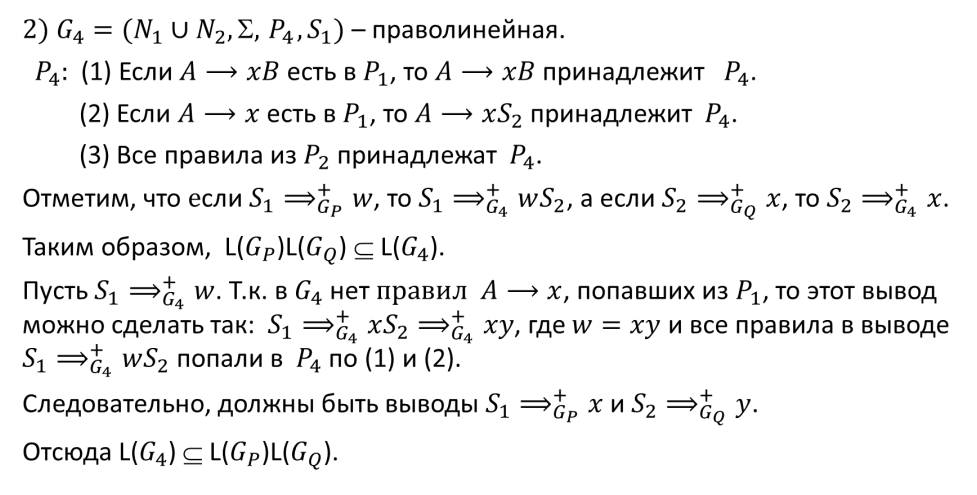
\includegraphics[width=1\linewidth]{Снимок экрана 2025-03-06 083127.png}
\end{figure}


\begin{figure}[H]
    \centering
    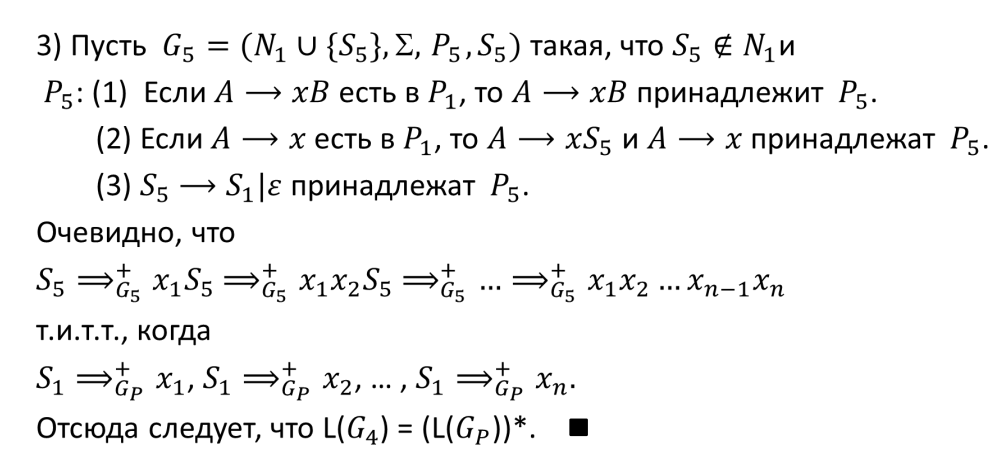
\includegraphics[width=1\linewidth]{Снимок экрана 2025-03-06 083156.png}
\end{figure}


• Теорема. Язык является регулярным множеством т.и.т.т., когда он
праволинейный.

• Док-во.

Необходимость.

Следует из лемм 3 и 4, индукцией по числу шагов построения регулярного
множества, где один шаг – это применение одного из правил, определяющих
регулярные множества.

\begin{figure}[H]
    \centering
    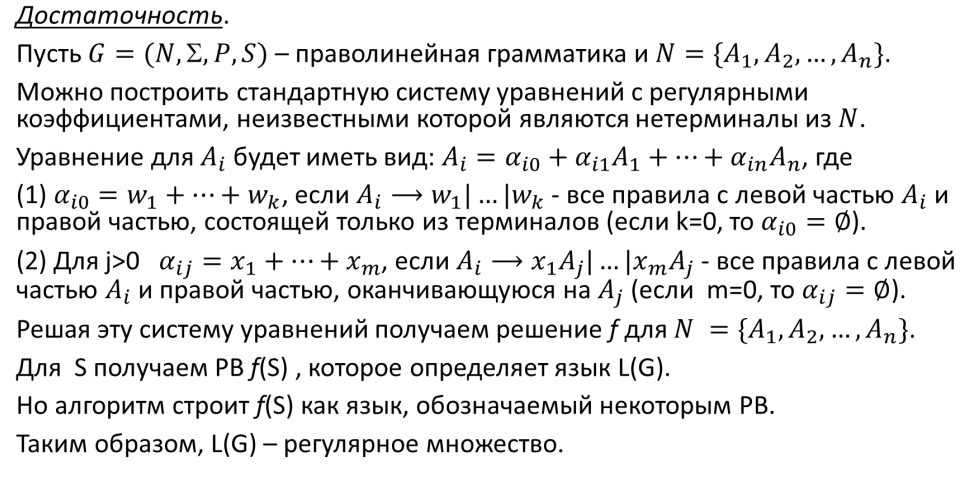
\includegraphics[width=1\linewidth]{Снимок экрана 2025-03-06 083319.png}
\end{figure}


\subsection{Пример построения грамматики по РВ}


\begin{figure}[H]
    \centering
    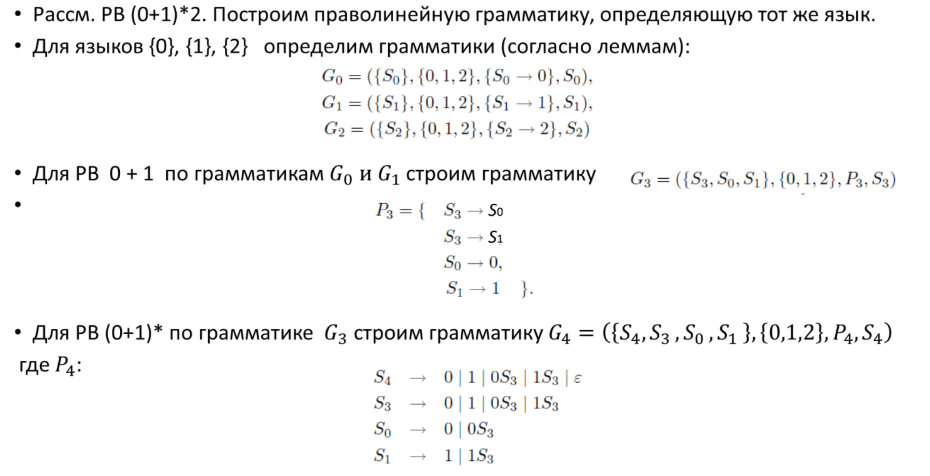
\includegraphics[width=1\linewidth]{Снимок экрана 2025-03-06 085249.png}
\end{figure}


Тут надо фотку доски вставить 

\begin{figure}[H]
    \centering
    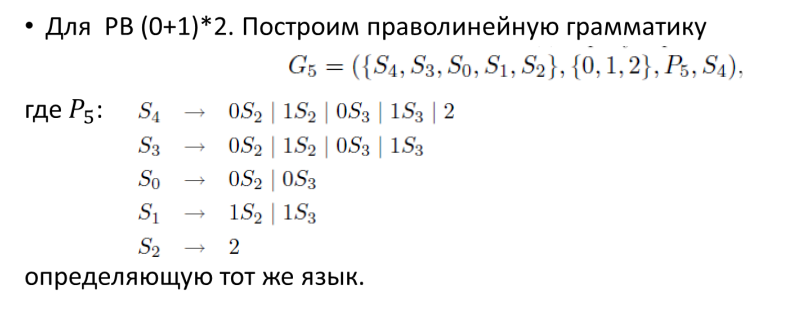
\includegraphics[width=1\linewidth]{Снимок экрана 2025-03-06 085516.png}
\end{figure}


\begin{figure}[H]
    \centering
    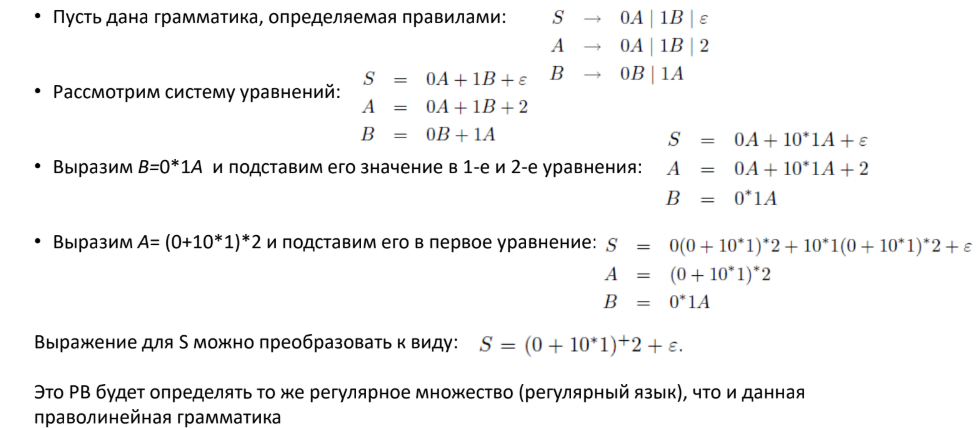
\includegraphics[width=1\linewidth]{Снимок экрана 2025-03-06 085735.png}
\end{figure}


\section{Конечные автоматы и регулярные множества}

\subsection{Способы определения класса регулярных множеств}

• Класс регулярных множеств – наименьший класс языков,
содержащий $\varnothing$, {$\epsilon$}. {$\alpha$} для всех a и замкнутый относительно
операций объединения, конкатенации и итерации.

• Регулярное множества – множества, определяемые регулярными
выражениями.

• Регулярное множества – языки, порождаемые праволинейными
грамматиками.

• Регулярное множества – языки, распознаваемые конечными
автоматами.

\textbf{Что такое конечный автомат?}

• Формальная система.

• Помнит только конечное количество информации.

• Информация представляется его состояниями.

• Состояние изменяется по воздействием входов.

• Правила, которые говорят, как изменять состояния под

воздействием входов, называются переходами.


\textbf{Допустимые входы}


• Дана последовательность входов (входная строка).

• Начать в начальном состоянии и следовать по переходу по
каждому очередному символу входной строки.

• Вход принимается, если вы перенеслись в финальное
(принимающее) состояние после чтения всех входных символов.

\textbf{Язык автомата}

• Множество строк, принимаемых автоматом A, являются языком
автомата A.

• Обозначается L(A).

• Различные множества финальных состояний -> Разные языки.


\subsection{Детерминированный конечный автомат}

!Нужно обзательно оьяснить функцию пперехода, без этого ответ не полный

\begin{figure}[H]
    \centering
    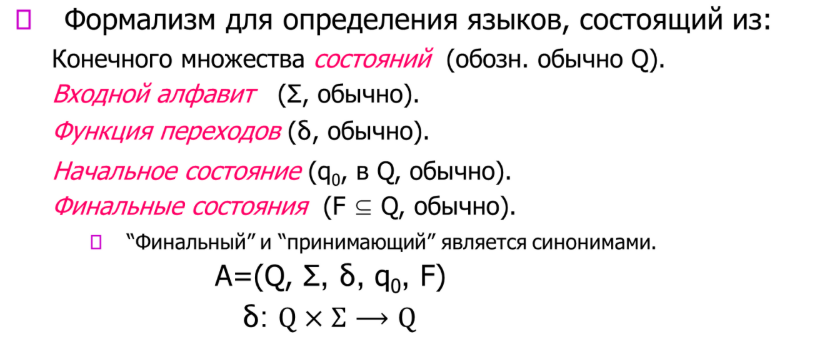
\includegraphics[width=1\linewidth]{Снимок экрана 2025-03-06 091303.png}
\end{figure}


\textbf{Функция переходов}



Имеет два аргумента: состояние и входной символ.

$\delta(q,a)$ = состояние, в которое КДА переходит, если он в
состоянии q получает на вход символ a.

Замечание: всегда есть следующее состояние – добавим
мёртвое состояние если нет переходов (Пример далее).

Форма задания: таблица переходов, граф.

Функцию переходов можно доопределить для слов:

$\delta*(q, a) = \delta(q,a)$  если |a|=1.

$\delta*(q, aw) = \delta(\delta*(q, w) , a)$

\begin{figure}[H]
    \centering
    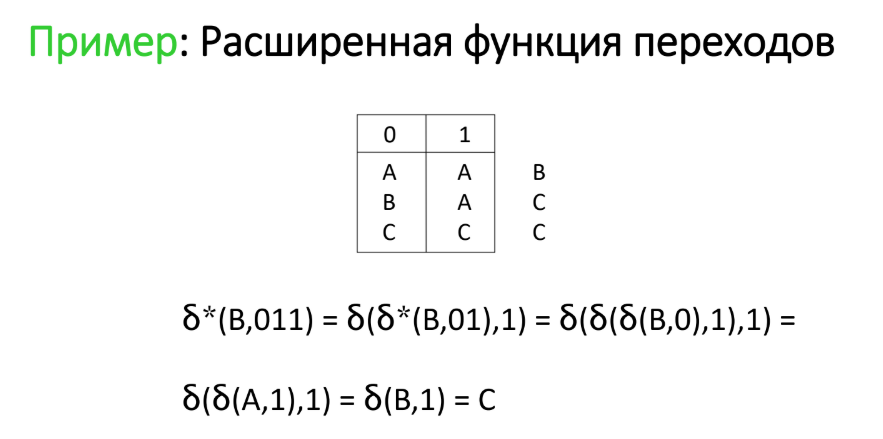
\includegraphics[width=1\linewidth]{Снимок экрана 2025-03-06 092352.png}
\end{figure}


\textbf{Дельта с крышкой}

Мы не будем различать обозначения

дельта и дельта со звездочкой

Причина:

$\delta*(q, a) = \delta(\delta*(q, \epsilon), a) = \delta(q, a)$

Расширенная дельта $\delta*$


\textbf{Представление КДА графом}

Вершины = состояния.

Дуги представляют функцию переходов.

Дуга из состояния p в состояние q помечается всеми
теми входными символами, по которым происходит
переход из p в q.

Стрелка помеченная как “Start” указывает на
начальное состояние.

Финальные состояния обозначаются двойной
окружностью.

\begin{figure}[H]
    \centering
    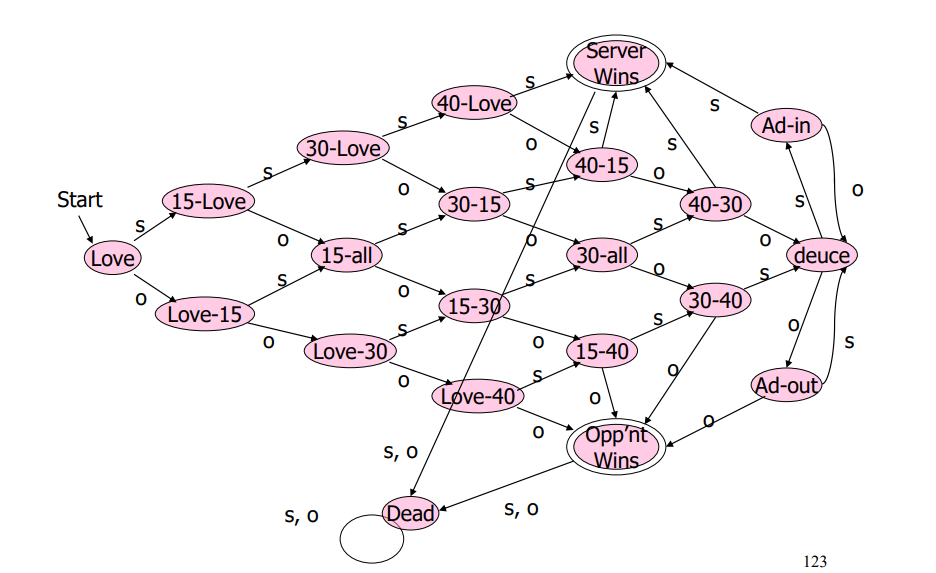
\includegraphics[width=1\linewidth]{Снимок экрана 2025-03-06 094224.png}
\end{figure}



\textbf{Соглашение: Строки и Символы}

… w, x, y, z - строки.

a, b, c,… - одиночные входные
символы.


\textbf{20.03.25}

\section{Недетерминнированный конечный автомат}

Недетерминированный конечный автомат может находиться
в нескольких состояниях одновременно.

Переходы из состояния по входному символу могут быть в
любое множество состояний.

Начать работу в начальном состоянии.

Принять, если какая-либо последовательность переходов
приводит в заключительное состояние.

Интуитивно: НКА всегда “угадывает правильно.”

\begin{figure}[H]
    \centering
    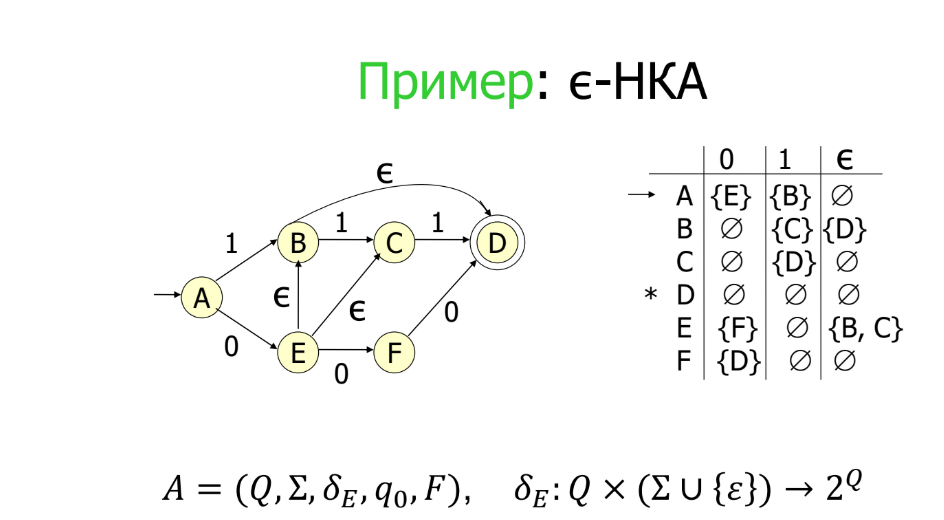
\includegraphics[width=1\linewidth]{Снимок экрана 2025-03-20 082634.png}
\end{figure}


\textbf{Эквивалентность НКА, $\epsilon$ - НКА}


Каждый НКА является $\epsilon$-НКА.

Он только не имеет $\epsilon$-переходов.

Доказательство обратного требует от нас взять
$\epsilon$-НКА и построить НКА, который принимает тот
же язык.

Мы сделаем это путем комбинирования
$\epsilon$–переходов со следующим переходом по
реальному входу.

\begin{figure}[H]
    \centering
    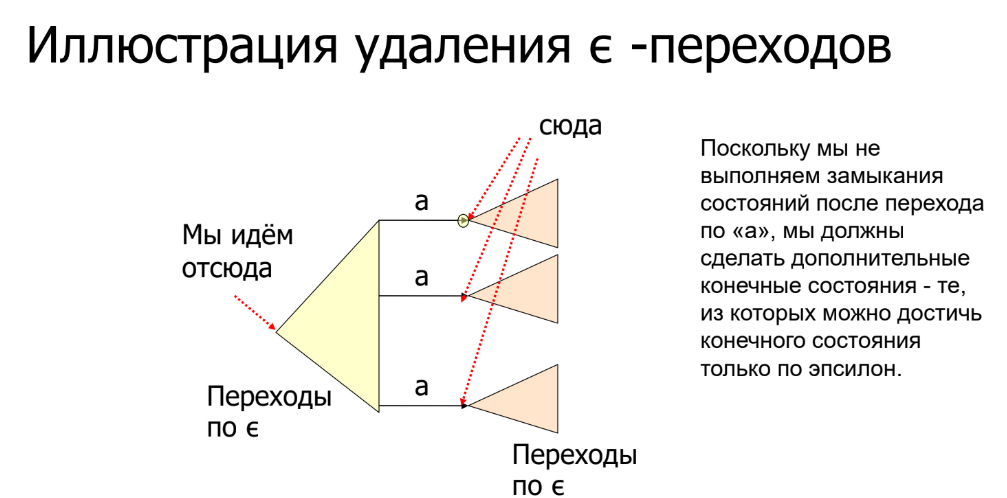
\includegraphics[width=1\linewidth]{Снимок экрана 2025-03-20 082840.png}
\end{figure}

\begin{figure}[H]
    \centering
    \includegraphics[width=1\linewidth]{Снимок экрана 2025-03-20 083112.png}
\end{figure}

\begin{figure}[H]
    \centering
    \includegraphics[width=1\linewidth]{Снимок экрана 2025-03-20 083123.png}
\end{figure}


\textbf{Эквивалентность – (4)}

Доказательство индукцией по |w| того, что

CL($\delta_N(q_0,w)) = \widehat{\delta}_E(q_0,w)$. (1)

Идея доказательства: НКА на любом входе w переходит в тот же набор
состояний, в который переходит $\epsilon$-НКА на том же входе, используя, где
возможно, $\epsilon$- переходы, кроме как в конце - после чтения всех реальных
входов w. Однако, состояние p в E
$\widehat{\delta}_E(q_0,w)$ является конечным состоянием,
если в $\epsilon$-НКА из p можно достичь конечного состояния, следуя только по $\epsilon$.
Таким образом, тот факт, что равенство (1) выполняется, означает, что w
принимается или не принимается обоими автоматами; то есть они
принимают один и тот же язык.
Т.о., $\epsilon$-НКА принимает w т.и т.т., когда его принимает "обычный"
НКА.

\begin{figure}[H]
    \centering
    \includegraphics[width=1\linewidth]{Снимок экрана 2025-03-20 083857.png}
\end{figure}



\textbf{Заключение}

Теорема. КДА, НКА, и $\epsilon$–НКА все принимают в точности
одно и то же множество языков: регулярные языки.

По этой причине эти языки ещё называют автоматными.

Типы НКА проще строить и они могут иметь
экспоненциально меньше состояний, чем КДА.

Но только КДА может быть реализован!

\subsection{Эквивалентность РВ и конечных автоматов}

Теорема. Регулярные выражения и конечные автоматы
представляют один и тот класс регулярных языков.

Нужно показать, что для каждого РВ существует конечный
автомат, который принимает тот же самый язык, что
определяет РВ.

Для доказательства возьмём наиболее мощный тип
автомата: $\epsilon$-НКА.

Также, нужно показать, что для каждого конечного автомата
существует РВ, определяющее тот же язык, что КА
Для доказательства выберем наиболее ограничительный
тип: КДА.


\subsection{Преобразование РВ в $\epsilon$-НКА}

Докажем индукцией по числу операторов
(+, конкатенация, *) в РВ.

Мы всегда строим автомат специального вид.

\textbf{Вид построенного $\epsilon$ НКА}

\begin{figure}[H]
    \centering
    \includegraphics[width=1\linewidth]{Снимок экрана 2025-03-20 085148.png}
\end{figure}


\textbf{От РВ к $\epsilon$-НКА: Базис}

\begin{figure}[H]
    \centering
    \includegraphics[width=1\linewidth]{Снимок экрана 2025-03-20 085218.png}
\end{figure}

\textbf{От РВ к $\epsilon$-НКА: Индукция 3 – Объединение}

\begin{figure}[H]
    \centering
    \includegraphics[width=1\linewidth]{Снимок экрана 2025-03-20 085605.png}
\end{figure}


\subsubsection{Примеры}

\textbf{Пример построения КА по PB}

 Регулярное выражение: (a+b)(cd)*

 1) Автоматы для РВ a, b, c, d

 \begin{figure}[H]
    \centering
    \includegraphics[width=0.30\linewidth]{Снимок экрана 2025-03-20 085702.png}
\end{figure}

\textbf{Пример построения КА по PB (2)}

\begin{figure}[H]
    \centering
    \includegraphics[width=1\linewidth]{Снимок экрана 2025-03-20 085742.png}
\end{figure}

\textbf{Пример построения КА по PB (3)}

\begin{figure}[H]
    \centering
    \includegraphics[width=1\linewidth]{Снимок экрана 2025-03-20 090034.png}
\end{figure}


\textbf{Пример построения КА по PB (4)}

\begin{figure}[H]
    \centering
    \includegraphics[width=1\linewidth]{Снимок экрана 2025-03-20 090047.png}
\end{figure}


\subsection{От-ДКА-к-PB}

Необычный вид индуции.

Пусть состояния КДА именуюутся 1,2,...,n.

Индукция проводится по k, максимальному числу
состояний, по которым нам позволено проходить вдоль
пути.


\subsection{k-Пути}

K-путь – это путь в графе КДА, который не проходит
через состояния с номерами больше, чем k.

Выбор конечной вершины не ограничивается; ей может
быть любое состояние.

n-пути являются неограниченными (n – число состояний
автомата).

РВ есть объединение РВ для n-путей от начального
состояния к каждому конечному состоянию.

\textbf{Пример: k-пути}

\begin{figure}[H]
    \centering
    \includegraphics[width=1\linewidth]{Снимок экрана 2025-03-20 091100.png}
\end{figure}

\textbf{Промежуточные итоги}

Каждый из рассмотренных трёх типов автоматов
(КДА, НКА, $\epsilon$-НКА), а также регулярные
выражения, определяют одно и то же множество
языков: регулярные языки.

РВ -> $\epsilon$-НКА -> НКА -> ДКА -> РВ


\subsection{Эквивалентность автоматных и
праволинейных языков}

\begin{figure}[H]
    \centering
    \includegraphics[width=0.50\linewidth]{Снимок экрана 2025-03-20 091416.png}
\end{figure}

\begin{figure}[H]
    \centering
    \includegraphics[width=0.50\linewidth]{Снимок экрана 2025-03-20 092027.png}
\end{figure}

\begin{figure}[H]
    \centering
    \includegraphics[width=0.50\linewidth]{Снимок экрана 2025-03-20 092811.png}
\end{figure}

Теорема. Язык праволинейный тогда и только тогда, когда
он автоматный.

 Доказательство следует из двух предыдущих лемм.

 \textbf{Заключение}


 Каждый из рассмотренных трёх типов автоматов (КДА, НКА, $\epsilon$-
НКА), а также регулярные выражения, определяют одно и то же
множество языков: регулярные языки.
Теорема. Утверждения:

 L – регулярный язык (регулярное множество),

 L – праволинейный язык,

 L – конечно-автоматный язык,

 L – недетерминированный конечно-автоматный язык,

 L обозначается (определяется) регулярным выражением
эквивалентны.

РВ -> $\epsilon$-НКА -> НКА -> ДКА -> РВ

\begin{figure}[H]
    \centering
    \includegraphics[width=0.50\linewidth]{Снимок экрана 2025-03-20 093221.png}
\end{figure}

\section{Свойста регулярных выражений}
\textbf{Свойста класса языков}

Класс языков - это множество языков.

Пример: регулярные языки.

Классы языков имеют два вида важных свойств:

1. Разрешимые свойства.

2. Свойства замкнутости.

\textbf{Свойства замкнутости}

Свойство замкнутости класса языков говорит, что выполнение
некоторой операции над языками в классе (например,
объединение) даёт в результате язык из того же класса.

Пример: регулярные языки, очевидно, замкнуты относительно
операций объединения, конкатенации и замыкания Клини
(данные операции называются регулярными).
Использовать для доказательства представление регулярных языков
регулярными выражениями.

\textbf{Представление языков}

Представление может быть формальным и неформальным.
Пример: (формальный): представление языка РВ или КДА,
определяющим соотв. язык.

Пример: (неформальный): логическое или описательное
утверждение о его строках:

{$0^n1^n|n$ неотрицательное число}

"Множество строк, состоящих из некоторого числа 0-ей, за которыми
следует такое же число 1."

\textbf{Разрешимое свойство}

Разрешимое свойство для класса языков – это алгоритм,
который по формальному описанию языка (например, КДА)
определяет выполнение или невыполнение некоторого
свойства.

Пример: Является ли язык L пустым?

\textbf{Почему важны разрешимые
свойства?}

Рассмотрим КДА, представляющий некоторый протокол.
Пример: “Завершается ли протокол?” = “Является ли язык
конечным?”

Пример: “Может ли протокол быть неверным?” = “Является ли
язык непустым?”

Сделать финальным состоянием “состояние ошибки”.

Нам хотелось бы иметь “наименьшее” представление языка, т.е.,
КДА с минимальным числом состояний или самое короткое РВ.

Можем ли мы определить, “Являются ли два языка одним и тем
же?”
Т.е., определяют ли два КДА один и тот же язык?
 
\textbf{Проблема принадлежности
строки языку}

Нашей первой разрешимой проблемой для регулярных
языков будет ответ на вопрос: “находится ли строка w в
регулярном языке L?”

Предположим, что L представлен КДА A.

Смоделируем работу A на последовательности входных
символов w.

\textbf{27.03.25}



\section{Свойста регулярных языков}

\textbf{Свойства класса языков}

Класс языков - это множество языков.

Пример: регулярные языки.

Классы языков имеют два вида важных свойств:

1. Разрешимые свойства.

2. Свойства замкнутости.


\textbf{Свойство замкнутости}

Свойство замкнутости класса языков говорит, что выполнение
некоторой операции над языками в классе (например,
объединение) даёт в результате язык из того же класса.

Пример: регулярные языки, очевидно, замкнуты относительно
операций объединения, конкатенации и замыкания Клини
(данные операции называются регулярными).

Использовать для доказательства представление регулярных языков
регулярными выражениями.

\textbf{Представление языков}



Представление может быть формальным и неформальным.
Пример: (формальный): представление языка РВ или КДА,
определяющим соотв. язык.
Пример: (неформальный): логическое или описательное
утверждение о его строках:

${0_n1_n | n – \text{неотрицательное число}}$

“Множество строк, состоящих из некоторого числа 0-ей, за которыми
следует такое же число 1.”



\textbf{Разрешимое свойство}

Разрешимое свойство для класса языков – это алгоритм,
который по формальному описанию языка (например, КДА)
определяет выполнение или невыполнение некоторого
свойства.

Пример: Является ли язык L пустым?

\textbf{Проблема пустоты}

Для данного регулярного языка определить, содержит ли он
хотя бы одну строку ?

Пусть предсталением языка является КДА.

Вычислим множество состояний, достижимых из
начального.

Если хотя бы одно из конечных состояний достижимо, то
ответ “да”, иначе - “нет”.

Проблема пустоты для регулярных языков разрешима.


\textbf{Проблема бесконечности}


Является данный регулярный язык бесконечным?
Рассмотрим КДА для языка.

Ключевая идея: если КДА имеет n состояний и язык содержит
какую либо строку длины n или более, то язык бесконечный.

В противном случае, язык, безусловно, конечный.

Можно ограничиться строками длины n или меньше.


\textbf{03.04.25}

\subsection{Разрешимые свойства для регулярных языков - итоги}


\textbf{Слудующие проблемы разрешимы для регулярных язков:}

Проблема принадлежности языку: w $\in$ L?

 Проблема пустоты: L=$\varnothing$?

 Проблема эквивалентности: L = M?

 Проблема вложения языков: L $\subseteq $ M?

 Проблема бесконечности языка: |L| = $\infty$?

 \section{Свойства замыкания регулярных язков}

 \textbf{Свойства замкнутости}


 Свойство замкнутости класса языков говорит, что выполнение
некоторой операции над языками в классе (например,
объединение) даёт в результате язык из того же класса.

Пример: регулярные языки, очевидно, замкнуты относительно
операций объединения, конкатенации и замыкания Клини
(данные операции называются регулярными).

Использовать для доказательства представление регулярных языков
регулярными выражениями.


\textbf{Замкнутость класса регулярных языков относительно регулярных операций}


\begin{figure}[H]
    \centering
    \includegraphics[width=1\linewidth]{Снимок экрана 2025-04-03 083232.png}
\end{figure}

\subsection{Замыкание по конкатенации и операции Клини}

Та же идея:

RS — РВ, языком для которого является язык LM.

R* — РВ, языком для которого является язык L*.


\subsection{Замыкание по пересечению}

Теорема. Если L и M – регулярные языки, то таковым
будет язык L $\cap $ M.

Доказательство: Пусть A и B – КДА, определяющие языки
L и M, соотвественно.

Построим автомат C – произведение автоматов A и B.
Сделаем финальными состояниями C пары, состоящие из
финальных состояний A и B.

\begin{figure}[H]
    \centering
    \includegraphics[width=1\linewidth]{Снимок экрана 2025-04-03 083957.png}
\end{figure}

\textbf{Пример: Использование свойства замыкания пересечения}


Мы доказали с использованием леммы о накачке, что
$L_1$ = {$0^n1^n | n > 0$} - не регулярный язык.

$L_2$ = множество строк с равным числом 0 и 1 тоже не
РЯ, но этот факт трудно доказать напрямую.

Предположим, что L2 – регулярный язык.

Регулярные языки замкнуты относительно $\cap$.

Если $L_2$ регулярный, то $L_2$ $\cap$L(0*1*) = L1
тоже должен бы быть регулярным, но мы уже установили, что это не
так.

\subsection{Заымкание по вычитанию}

Теорема. Если L и M – регулярные языки, то таким является
язык L – M (строки из L, но не из M).

Доказательство: Пусть A и B - КДА, языками которых
являются L и M соотвественно.

Построим автомат C – произведение автоматов A и B.

Сделаем финальными состояниями автомата C пары,
которые состоят из финальных состояний A и нефинальных
B.

Автомат С допускает точно строки из L – M.
Следовательно, L – M – регулярный язык.


....


....


....
\subsection{Гомоморфизм}



тут где то должен посоедний слайд


\vspace{1cm}

\textbf{10.04.25}

\section{Контекстно-свободные грамматики}



Неформальные комментарии

• Контекстно-свободная грамматика – нотация для описания языков.
• Она более мощная, чем КДА или РВ, но не может определять все
возможные языки.

• Полезна для описания вложенных структур, т.е., скобок в языках
программирования.

• Основная идея использования «переменных» – для обозначения
множеств строк (т.е., языков).

• Эти переменные определяются рекурсивно, в терминах друг друга.

• Рекурсивные правила (“продукции”) включают только конкатенацию.

• Альтернативные правила для переменных допускают объединение.



\textbf{Грамматики}


Порождающая грамматика G — это четверка $\langle T, N, P, S  \rangle $,
где T — алфавит терминальных символов ( терминалов );
N — алфавит нетерминальных символов (нетерминалов), $T \bigcap N =\varnothing$;
P — конечное подмножество множества $(T \bigcup N)^+ (T \bigcup N)^*$

Пара $(\alpha, \beta)\in P$ (записывается в виде $\alpha -> \beta$) называется правилом вывода;
a называется левой частью (головой) правила, b — правой частью (телом)
правила.

Левая часть любого правила из P обязана содержать хотя бы один
нетерминал;
S — начальный символ грамматики, $S \in N$.
Для записи правил вывода с одинаковыми левыми частями

$\alpha -> \beta_1 \alpha -> \beta_2 ... \alpha -> \beta_n$

используют сокращенную запись $\alpha -> \beta_1 | \beta_2 |...| \beta_n$

\textbf{Классификация грамматик и языков по Хомскому: Тип 2}

Грамматика G = $ \langle T, N, P, S \rangle $ называется контекстно-
свободной (КС), если каждое правило из Р имеет вид A -> B, где

$A \in N, B \in ( T \cup N )^*$

Заметим, что в КС-грамматиках допускаются правила с пустыми
правыми частями. Язык, порождаемый контекстно-свободной
грамматикой, называется контекстно-свободным языком.


\vspace{1cm}

\textbf{17.04.25}


\textbf{Дерево вывода}

Опр. Помеченное упорядоченное дерево D называется деревом
вывода (или деревом разбора) в КС-грамматике G = (N, $\Sigma $, P, S), если
выполнены следующие условия:

1. Корень дерева D помечен S.

2. Каждый узел имеет метку из N $\cup $ $\Sigma$ $\beta \cup$ {$\varepsilon$}

3. Если узел имеет хотя бы одного потомка, метка этого узла –
нетерминальный символ

4. Если $D_1,D_2 , ... ,D_k$ - поддеревья с корнями $X_1, X_2 , ... , X_k$, которые
являются прямыми потомками, то в множестве правил P
присутствует правило $X_2 ... X_k$ . При этом поддерево Di может быть
узлом с меткой корня $X_i$ = $\varepsilon $ только в случае, 
если $X_i$ - единственный
потомок узла А и в P присутствует правило $A \rightarrow  \varepsilon$.




\textbf{Неоднозначность, – (2)}


Таким образом, эквивалентным определением для
“неоднозначной грамматики’’ служит:

1. Существует строка языка, которая имеет два различных левых вывода.

2. Существует строка языка, которая имеет два различных правых
вывода.


тут еще должно пара слайдов


\section{Нормальные формы КС-грамматик}

\textbf{КС-грамматики и $\varepsilon$ - правила}

Опр. Грамматика G =$\langle  T, N, P, S \rangle $ азывается контекстно-
свободной (КС), если каждое правило из Р имеет вид A $\to$ b, где

$A \in N, \beta \in ( T \cup N )*.$

В КС-грамматиках допускаются правила с пустыми правыми
частями.
Язык, порождаемый контекстно-свободной грамматикой,
называется контекстно-свободным языком.


Переменные из которых ничего не выводиться

Рассмотрим грамматику с правилами:

$ S \rightarrow AB,
\vspace{3mm}
 A \rightarrow  aA | a,
\vspace{3mm}
 B \rightarrow AB$

 Хотя A выводит все строки над алфавитом {a}, B не выводит
терминальных строк.

 Почему? Единственная продукция для B оставляет B в сентенциальной
форме.

 Таким образом, S не выводит ничего, и соответствующий язык
пуст.


Упрощающие алгоритмы


Есть целое семейство алгоритмов, которые работают по
индуктивному принципу.

 Они начинают с открытия (констатации) некоторых
очевидных фактов, (базис).

 Они открывают больше фактов из тех, которые уже
открыты (индукция).

 В конце концов, когда ничего больше не может быть
обнаружено, мы заканчиваем.


\textbf{Проверка выводимости некоторой
терминальной строки из переменной}

 Базис: Если есть правило A => w, где w не имеет переменных, то A
выводит терминальную строку (из нетерминального символа А
выводится терминальная цепочка символов).

 Индукция: Если есть правило A => a, где a состоит только из
терминалов и переменных, о которых известно, что они выводят
терминальные строки. Тогда A выводит терминальную строку.

 Мы оканчиваем процесс, когда не можем найти новых переменных.

 Простая индукция по порядку, в котором находятся переменные,
показывает, что каждая из них действительно выводит терминальную
строку.

 Обратно, любая переменная, которая выводит терминальную строку,
может быть найдена приведенным алгоритмом.


\textbf{Алгоритм удаления переменных, из которых
ничего не выводится}

1. Найдём все переменные, из которых выводятся
терминальные строки. Назовем такие переменные
полезными.

2. Для всех других переменных (бесполезных), удалим из
грамматики все правила, в которых они появляются либо
в голове, либо в теле.


Пример: Удаление переменных

$S \rightarrow AB | C, A \rightarrow aA | a, B \rightarrow bB, C \rightarrow c$

 Базис: A и C находятся, т.к. $A \rightarrow a$ и $ C \rightarrow c.$

 Индукция: S находится (помечается), т.к. $S \rightarrow C.$
 Больше ничего не находится.

 Результат:$ S \rightarrow C,$

 $A \rightarrow aA | a,$

 $C \rightarrow c$



Недостижимые символы

 Другой случай кандидата на удаление терминала или
переменной - если она не может появиться в каком-либо
выводе из начального символа.
 Базис: Мы всегда можем достичь S (начальный символ).
 Индукция: Если мы можем достичь A, и есть правило A => a,
то мы можем достичь a.

\textbf{Устранение недостижимых символов}
\begin{figure}[H]
    \centering
    \includegraphics[width=0.50\linewidth]{Снимок экрана 2025-04-17 084851.png}
\end{figure}



\textbf{Удаление бесполезных символов}

 Опр. Символ называется полезным, если он появляется в
некотором выводе какой-либо терминальной строки из
начального символа.

 В противном случае, он является бесполезным.

 Удалим все бесполезные символы:

 Идея алгоритма:

1) Удалим все символы, из которых не выводятся терминальные
строки.

2) Удалим недостижимые символы.


Пример: Бесполезные символы – важен порядок удаления(2)

S -> AB, A -> C, C -> c, B -> bB

 Как и следует, мы сначала удаляем символы, из которых не
выводятся терминальные строки и соответствующие правила, т.е.
удаляем B.

 Но, удалив B, мы удаляем правило B -> bB, а затем и правило
вывода из начального символа S -> AB.

 Затем, мы применяем алгоритм поиска недостижимых символов
из начального и видим, что всё недостижимо, т.е. все правила
будут удалены.

 Однако, если мы сначала будем удалять недостижимые символы,
то увидим, что всё достижимо из S, т.е. ничего не удалиться.

 Т.о. A, C, и c никогда не будут удалены, останутся правила A -> C,
C -> c, которых не должно быть, т.к. A, C, и c – бесполезные.


\textbf{Разрешимость проблемы пустоты
КС-грамматик}




\textbf{Устранение бесполезных символов}




тут куча должна быть всего


Единичные правила-(2)



тут тоже много всего

Одно из приложений НФХ


\vspace{5mm}

\textbf{15.05.25}

\section{Автоматы с магаизной паматью}


Автоматы с магазинной памятью


• МП-автомат – это автомат эквивалентный по своей
выразительной мощности определения КС-языков.

• Только недетерминированные МП-автоматы определяют все
КС-языки.

• Но детерминированная версия моделирует синтаксические
анализаторы.

• Большинство языков программирования имеют детерминированные
МП-автоматы.


МПА формально

• МПА определяется: $(Q, \Sigma , \Gamma , \delta , q_0, Z_0, F)$

1. Конечным множеством состояний (Q, обычно).

2. Входным алфавитом $(\Sigma, $обычно).

3. Алфавитом стека ($\Gamma,$ обычно).

4. Функцией переходов $(\delta,$ обычно).

5. Начальным состоянием $(q_0,$ в Q, обычно).

6. Начальным символом $(Z_0, в \Gamma$, обычно).

7. Множеством конечных состояний $(F \subseteq  Q,$ обычно).

Мгновенная конфигурация

• Мы можем формализовать описание работы МПА на основе

мгновенных конфигураций (ID- instantaneous description).
• ID – это тройка (q, w, a), где:

1. q – текущее состояние.

2. w – оставшийся непрочтенный вход.

3. a - содержимое стека, с вершиной слева.

\section{Эквивалентность МП-автоматов и КС-грамматик}

\section{Лемма о накачке для КС-языков}


\section{Свойства КС-языков}

Обзор разрешимых свойств

• Обычно, когда мы говорим о КС-языках , мы имеем в виду их
представление в виде КС-грамматики или МП-автомата,
принимающих строки по переходу в конечное состояние или
опустошением стека.

• Существуют алгоритмы решающие:

1. Принадлежит ли строка w КС-языку L.

2. Является ли КС-язык пустым.

3. Является ли КС-язык бесконечным.

Неразрешимые свойства

• Многие вопросы, разрешимые для регулярных языков, не
могут быть разрешимы для КС-языков.

• Пример: Являются ли два КС-языка одним и тем же?

• Пример: Являются ли два КС-языка несвязными (пересечение
пусто)?

• Как бы вы это сделали для регулярных языков?

• Нужна теория машин Тьюринга и неразрешимых задач, чтобы
доказать отсутствие соответствующих алгоритмов.

Проверка членства

• Необходимо узнать, принадлежит ли строка w языку L(G).
• Предположим G находится в НФХ.

• Или преобразуем данную грамматику в НФХ.

• w = $\varepsilon $ является специальным случаем, разрешаемым
посредством проверки того, является ли начальный символ
пустым.

• Алгоритм (CYK ) является хорошим примером
динамического программирования и работает время
порядка O($n^3$), где n = |w|.

CYK =John Cocke, Dan Younger, and Tadao Kasami



\vspace{5mm}

\textbf{22.05.25}


\section{Неразрешимость}






тут куча текста и прочего 



\textbf{Универсальный язык}





\end{document}
